%   Version 2.0 | Lehrstuhl Regelungstechnik & Mechatronik  |  15.05.2020
%%%%%%%%%%%Zusätzlich benötigte Pakete in den header einfügen%%%%%%%%%%%%
%   header.tex 
%   Version 1.0     |   Peter Krönes    |   08.05.2018
%%%%%%%%%%%%%%%%%%%%%%%%%%%%%%%%%%%%%%%%%%%%%%%%%%%%%%%%%%%%%%%%%%%%%%%%
\documentclass
[   oneside,         % oneside/twoside : Einseitiger oder zweiseitiger Druck?
    12pt,            % Bezug: 12-Punkt Schriftgröße
    DIV=15,          % Randaufteilung, siehe Dokumentation "KOMA"-Script
    BCOR=17mm,       % Bindekorrektur: Innen 17mm Platz lassen. Copyshop-getestet.
    headsepline,     % Unter Kopfzeile Trennlinie (aus: headnosepline)
    openright,       % Neue Kapitel im zweiseitigen Druck rechts beginnen lassen
    a4paper,         % Seitenformat A4
    listof=totoc,      % Div. Verzeichnisse ins Inhaltsverzeichnis aufnehmen
    bibliography=totoc,        % Literaturverzeichnis ins Inhaltsverzeichnis aufnehmen
]   {scrbook}        %scrbook für Abschlussarbeiten 
%%%%%%%%%%%%%%%%%%%%%%%%%%%%%%%%%%%%%%%%%%%%%%%%%%%%%%%%%%%%%%%%%%%%%%%%%%%%%
\usepackage[
    backend=biber,
    natbib=true,
    url=false, 
    doi=true,
    eprint=false,
    backref=true
]{biblatex}
\usepackage{hyperref}%[pdftex,bookmarks,colorlinks,citecolor=black,breakl inks]
\appto\UrlBreaks{\do\a\do\b\do\c\do\d\do\e\do\f\do\g\do\h\do\i\do\j
	\do\k\do\l\do\m\do\n\do\o\do\p\do\q\do\r\do\s\do\t\do\u\do\v\do\w
	\do\x\do\y\do\z}						% Umbruch von langen URLs

\DefineBibliographyStrings{ngerman}{%
  backrefpage = {S.},                       % originally "cited on page"
  backrefpages = {S.},                      % originally "cited on pages"
  andothers = {{et\,al\adddot}},
}
%%%%%%%%%%%%%%%%%%%%%         PAKETE        %%%%%%%%%%%%%%%%%%%%%%%%%%%%
\usepackage[utf8]{inputenc} 
\usepackage{csquotes}                       % Anführungszeichen
\usepackage{setspace}                       % Zeilenabstand
\usepackage[ngerman]{babel}                 % Spracheinstellung
\usepackage{float}                          % Platzierung von Objekten
\floatstyle{plaintop}						% Caption über Tabellen
\restylefloat{table}						% ^^^^^^^^^^^^^^^^^^^^
\usepackage{pdfpages}                       % PDF Seitenweise einfügen
\usepackage[font=normalsize]{caption}       % Größe der Bild-/Tabellenunterschrift 
\usepackage{acronym}                        % Abkürzungsverzeichnis
\newcommand{\acrosecondcolumn}[1]{
  \acroextra{\makebox[70mm][l]{#1}}
}
\usepackage{graphicx}                       % Für Bilder
\usepackage{subcaption}                     % mehrere Bilder nebeneinander
\usepackage{floatflt}                       % Umlossene Bilder
%\usepackage{overpic}						% Überlagerung von Bildern
\usepackage{svg}                            % Vektorgrafiken im svg-format
%\usepackage{tabu}						    % Abstände in Tabellen (\tabulinesep)
\usepackage{tabularx}                       % Für Tabellen
\usepackage{booktabs}                       % Noch ein Tabellenpaket
\usepackage{color}                          % farbiger Text
\usepackage{lineno}                         % Zeilennummern 
\usepackage{microtype}                      % Macht alles schöner
\usepackage{listings}                       % Für Code
\usepackage{src/mcode/mcode}                % Matlab-Code Paket
\usepackage{src/abkuerzung}                 % Abkürzungen
\usepackage{blindtext}                      % Beispieltext zum auspobieren
\usepackage{todonotes}                      % Fügt Todo Notes ein
\usepackage{eurosym}                        % Eurozeichen mit \euro
\usepackage{afterpage}						% A3 pages in A4 Document
\usepackage[decimalsymbol=comma]{siunitx}   % SI-Einheiten
\usepackage{array}                          % Array


%% Tikz-Pakete
\usepackage{tikz}
\usepackage[siunitx,european,straightvoltages]{circuitikz}          % Schaltkreise
\usetikzlibrary{decorations.pathreplacing}                          % Schaltkreiszusatz
%\usetikzlibrary{arrows.meta}
\usetikzlibrary{arrows}
\usetikzlibrary{patterns}
\usetikzlibrary{ipe}
\usetikzlibrary{positioning}
%\usetikzlibrary{shapes.geometric}
\usetikzlibrary{shapes}
\usetikzlibrary{backgrounds}

%%Mathematik-Pakete für Formeln
\usepackage{amsmath}
\usepackage{amssymb}
\usepackage{amstext}
\usepackage{amsfonts}
\usepackage{mathrsfs}
\usepackage{mathtools}
%\usepackage{esvect}
%\numberwithin{equation}{section} %Nummerierungsebene für Gleichungen
\usepackage{gensymb}
\usepackage{multirow}
\usepackage{bigdelim}
\usepackage{epsfig}
\usepackage{etoolbox} 
\makeatletter 
\patchcmd\Gread@eps{\@inputcheck#1 }{\@inputcheck"#1"\relax}{}{}
\makeatother
%\renewcommand*{\familydefault}{\sfdefault}
%\newcommand*{\head}{\bfseries}
%
\newcolumntype{_}{>{\global\let\currentrowstyle\relax}}
\newcolumntype{^}{>{\currentrowstyle}}
\newcommand{\rowstyle}[1]{\gdef\currentrowstyle{#1}%
	#1\ignorespaces
}

%%%%%%%%%%%%%%%%%%%%%%%%%%%%%%%%%%%%%%%%%%%%%%%%%%%%%%%%%%%%%%%%%%%%%%%% 
% Setzt die Kapitel im Anhang nicht ins Inhaltsverzeichnis, setzt man 
% Abbildungsverzeichnis und Tabellenverzeichnis hinter den Anhang erscheinen 
% diese Trotzdem im Inhaltsverzeichnis.
%\usepackage[toc,page]{appendix}
%%%%%%%%%%%%%%%%%%%%%%%%%%%%%%%%%%%%%%%%%%%%%%%%%%%%%%%%%%%%%%%%%%%%%%%%
\setlength{\parindent}{0pt}                 % Absätze nicht eingerückt
%% Änderungen Pauline %%%%%%%%%%%%%%%%%%%%%%
\usepackage{cleveref}						% ans Ende verschoben, da Kompilierungsfehler

% Styles um Code mit oder ohne Zeilennummerierung auszugeben
\lstdefinestyle{numbers}{numbers=left, stepnumber=1, numberstyle=\tiny, numbersep=10pt,xleftmargin=1.5em}
\lstdefinestyle{nonumbers}{numbers=none}

%% Glossaries für Symbolverzeichnis
\usepackage[acronym,automake]{glossaries}             
\usepackage{glossary-longbooktabs}

\newglossary[klg]{konstante}{koi}{kog}{Konstanten} 
\newglossary[slg]{symbol}{syi}{syg}{Symbole} 
\glsaddkey{unit}{\glsentrytext{\glslabel}}{\glsentryunit}{\GLsentryunit}{\glsunit}{\Glsunit}{\GLSunit}

\newglossarystyle{3colger}{%
    \setglossarystyle{longragged3col}% base this style on the list style
    \renewenvironment{theglossary}{% Change the table type --> 3 columns
     % compute the description width
        \settowidth{\dimen0}{Zeichen}%  % so viel Platz, wie "Zeichen" braucht
        \settowidth{\dimen2}{laaaaangeEinheit}%
        \setlength{\glsdescwidth}{\linewidth-\dimen0-\dimen2-6\tabcolsep}
        \begin{longtable}{p{\dimen0} p{\glsdescwidth} p{\dimen2}}}%
        {\end{longtable}}%
    %
% \renewcommand*{\glossaryheader}{%  Change the table header
%  \bfseries Zeichen & \bfseries Beschreibung & \bfseries Einheit \\
%           \hline
%   \vspace{0.05cm}
%   \endhead}
\renewcommand*{\glossentry}[2]{%  Change the displayed items
    \glstarget{##1}{\glossentryname{##1}} %
    &  \glossentrydesc{##1}
    & \glsunit{##1}  \tabularnewline
}
\renewcommand*{\glsclearpage}{}  % damit alles auf einer Seite bleibt
}
\makeglossaries                                   % activate glossaries-package
\newcommand{\symbolverzeichnis}{
\glsaddall
\setglossarysection{section}
\printglossary[type = symbol, style=3colger]
\printglossary[type = konstante, style=3colger]}                                                  %
%%%%%%%%%%%%%%%%%   Diesen Abschnitt anpassen!    %%%%%%%%%%%%%%%%%%%%%%%
% Arbeit
\newcommand{\artderausarbeitung}{Abschlussarbeit}
\newcommand{\titelderarbeit}{Implementierung und Evaluation impliziter numerischer Differentialgleichungslöser für MeshGraphNets}
\newcommand{\eingereicht}{20.\,02.\,2020}
% Autor
\newcommand{\namedesautors}{Tim Schneider}
% Lehrstuhl und Betreuer
\newcommand{\studiengang}{Ingenieurinformatik}
\newcommand{\lehrstuhl}{Regelungstechnik}
\newcommand{\fakultaet}{Fakultät für Angewandte Informatik}
\newcommand{\erstgutachter}{Prof.~Dr.-Ing.~habil.~Christoph Ament}
\newcommand{\zweitgutachter}{Prof.~Dr.-Ing.~Lars Mikelsons}
\newcommand{\betreuer}{Vorname Nachname}
%%%%%%%%%%%%%%%%%%%%%%%%%%%%%%%%%%%%%%%%%%%%%%%%%%%%%%%%%%%%%%%%%%%%%%%%%
%   pagestyle.tex 
%   Version 1.0     |   Peter Krönes    |   08.05.2018

%%%%%%%%%%%%%%%%%%%%%%%  PAGESTYLE  %%%%%%%%%%%%%%%%%%%%%%%%%%%%%%%%%%%%

\usepackage{fancyhdr}
\pagestyle{fancy}
\renewcommand{\chaptermark}[1]{\markboth{ 
\thechapter. #1}{}}
\renewcommand{\sectionmark}[1]{\markboth{ 
\thesection. #1}{}}
\fancypagestyle{scrheadings}{
   \fancyhead[LE,RO]{\pagemark}
   \fancyhead[LO]{\nouppercase\leftmark}
   \fancyhead[RE]{\nouppercase\leftmark}
   \fancyfoot[C]{}
}

\fancypagestyle{plain}{%
\fancyhf{}
\renewcommand{\headrulewidth}{0pt}
\fancyhead[LE,RO]{\pagemark}
}
%%%%%%%%%%%%%%%%%%%%%%%%%%%%%%%%%%%%%%%%%%%%%%%%%%%%%%%%%%%%%%%%%%%%%%%%
% Pagestyle für die erste Seite der List of Figures/Tables
\fancypagestyle{pagenumberstyle}{
\renewcommand{\headrulewidth}{0pt}
\fancyhead[LE,RO]{\pagemark} %Seitenzahl oben-rechts
\fancyhead[L]{} %kein Kapitelname oben-links
\fancyfoot[C]{} %keine Seitenzahl unten
}
% Unterscheidung zwischen einseitig und zweiseitigem Druck nicht nötig, da Kapitel bei zweiseitigem Druck immer rechts anfangen.
%%%%%%%%%%%%%%%%%%%%%%%%%%%%%%%%%%%%%%%%%%%%%%%%%%%%%%%%%%%%%%%%%%%%%%%%

%%%%%%%%%%%%%%%%%%%%%%%%%%%%%%%%%%%%%%%%%%%%%%%%%%%%%%%%%%%%%%%%%%%%%%%%
% Pagestyle für scrartcl
\fancypagestyle{articlestyle}{
\renewcommand{\headrulewidth}{0.1pt}
\fancyhead[R]{\pagemark} %Seitenzahl oben-rechts
\fancyhead[L]{} %kein Kapitelname oben-links
\fancyfoot[C]{} %keine Seitenzahl unten
}
% Unterscheidung zwischen einseitig und zweiseitigem Druck nicht nötig, da Kapitel bei zweiseitigem Druck immer rechts anfangen.
%%%%%%%%%%%%%%%%%%%%%%%%%%%%%%%%%%%%%%%%%%%%%%%%%%%%%%%%%%%%%%%%%%%%%%%%
   % Pagestyles nicht verändern!               %
\addbibresource{src/references.bib}                                     %
%%%%%%%%%%%%%%%%%%%%%%%%%%%%%%%%%%%%%%%%%%%%%%%%%%%%%%%%%%%%%%%%%%%%%%%%%
% Hier können eigene Befehle angelegt werden:
%\newcommand{\Name}{Definition}
%%%%%%%%%%%%%%%%%%%%%%%%%%%%%%%%%%%%%%%%%%%%%%%%%%%%%%%%%%%%%%%%%%%%%%%%%    
\begin{document}                                                        %
\onehalfspacing                                                         %    
%   titlepage.tex 
%   Version 1.0     |   Peter Krönes    |   08.05.2018
\begin{titlepage}
\centering

\includegraphics[scale=0.4]{src/Uni_Aug_Logo_Basis_pos_A.pdf}\\[3ex]
{\Large \textsc{Universität Augsburg}}\\[3ex]
{\Large Fakultät für Angewandte Informatik}\\[3ex]
\vfill
{\Large \textbf{\artderausarbeitung}}\\[5ex]
{\large \textbf{\titelderarbeit}}\\[5ex]
\vfill
\begin{tabular}{rl}
\hline\\
vorgelegt von:          & \quad \namedesautors\\[1,5ex]
eingereicht am:         & \quad \eingereicht\\[1,5ex]
Studiengang:            & \quad \studiengang\\[1,5ex]

Anfertigung am Lehrstuhl:
                        & \quad \lehrstuhl\\[1,5ex]
                        & \quad \fakultaet\\[1,5ex]
1. Gutachter:
                        & \quad \erstgutachter\\[1,5ex]
2. Gutachter:
                        & \quad \zweitgutachter\\[1,5ex]
Wissenschaftlicher Betreuer:
                        & \quad \betreuer
\end{tabular}
\vfill
\end{titlepage}                                               %
\pagestyle{scrheadings}                                                 %
\pagenumbering{Roman}                                                   %
%%%%%%%%%%       Nicht benötigte Teile auskommentieren    %%%%%%%%%%%%%%%
\chapter*{Vorwort}
Diese LaTex-Vorlage dient der technischen und inhaltlichen Unterstützung wissenschaftlicher Arbeiten an den Lehrstühlen der Ingenieurinformatik. Kapitel \ref{ch:Wissenschaftliche_Arbeiten} gibt eine kurze Einführung in das wissenschaftliche Arbeiten und dabei zu beachtende formale und inhaltliche Aspekte. Die folgenden Kapitel geben eine technische LaTex-Einführung. Die dort präsentierten Vorlagen können in der wissenschaftlichen Arbeit genutzt werden.

Wenn man kein Vorwort benötigt, kann man den Befehl \verb+\chapter*{Vorwort}
Diese LaTex-Vorlage dient der technischen und inhaltlichen Unterstützung wissenschaftlicher Arbeiten an den Lehrstühlen der Ingenieurinformatik. Kapitel \ref{ch:Wissenschaftliche_Arbeiten} gibt eine kurze Einführung in das wissenschaftliche Arbeiten und dabei zu beachtende formale und inhaltliche Aspekte. Die folgenden Kapitel geben eine technische LaTex-Einführung. Die dort präsentierten Vorlagen können in der wissenschaftlichen Arbeit genutzt werden.

Wenn man kein Vorwort benötigt, kann man den Befehl \verb+\chapter*{Vorwort}
Diese LaTex-Vorlage dient der technischen und inhaltlichen Unterstützung wissenschaftlicher Arbeiten an den Lehrstühlen der Ingenieurinformatik. Kapitel \ref{ch:Wissenschaftliche_Arbeiten} gibt eine kurze Einführung in das wissenschaftliche Arbeiten und dabei zu beachtende formale und inhaltliche Aspekte. Die folgenden Kapitel geben eine technische LaTex-Einführung. Die dort präsentierten Vorlagen können in der wissenschaftlichen Arbeit genutzt werden.

Wenn man kein Vorwort benötigt, kann man den Befehl \verb+\include{001_Vorwort.tex}+ in der Main-Datei auskommentieren.
\cleardoublepage+ in der Main-Datei auskommentieren.
\cleardoublepage+ in der Main-Datei auskommentieren.
\cleardoublepage
\chapter*{Kurzfassung}

Diese Arbeit demonstriert, wie es möglich ist, implizite Differenzialgleichungslöser 
auf der Grafikkarte für \textit{MeshGraphNets} zu verwenden.
Ein \textit{MeshGraphNet} besteht dabei aus drei Komponenten.
Einer Gitterstruktur, die die diskreten Messpunkte der Simulation darstellen.
Einem Graphen, der dazu genutzt wird, Informationen zwischen den einzelnen gitter punkten im Mesh auszutauschen
und einem neuronalen Netzwerk, dass den nächsten Zeitschritt vorher sagt.
Um das neuronale Netzwerk mit einer erhöten Genauigkeit auswerten zu können, soll ein impliziter Differenzialgleichungslöser verwendet werden.
Das Lösen von impliziten verfahren setzt jedoch voraus, dass die Implementierung des neuronalen
Netzes automatisch abgeleitet werden kann.
In der Implementierung der \textit{MeshGraphNets} wird die \textit{scatter} Funktion verwendet, um Informationen
innerhalb der Graphdarstellung zwischen den einzelnen Knoten zu propagieren.
Diese kann jedoch keine \textit{Dual}-Zahlen verarbeiten, was die Grundlage für die automatische Differenzierung ist.
In dieser Arbeit wird demonstriert, wie diese Funktion so modifiziert werden kann, dass dies doch möglich ist.
Anschließend wird der Effekt der impliziten Löser auf die Genauigkeit und Laufzeit der MeshGraphNets betrachtet.

\cleardoublepage
%%%%%%%%%%%%%%%%%%%%%%%%%%%%%%%%%%%%%%%%%%%%%%%%%%%%%%%%%%%%%%%%%%%%%%%%%
\tableofcontents{\thispagestyle{pagenumberstyle}}                       %
\chapter*{Symbolverzeichnis}
\addcontentsline{toc}{chapter}{Symbolverzeichnis}
Einträge werden an beliebiger Stelle erzeugt mit \begin{verbatim}
    \newglossaryentry{c}{
    name=\ensuremath{c},
    description={Lichtgeschwindigkeit},
    unit={\SI{299792458}{\metre\per\second}},
    type=konstante}
\end{verbatim}
Als type lässt sich entweder \textit{symbol} oder \textit{konstante} wählen. 
Im Header können die Werte von \verb+\dimen0+ und \verb+\dimen2+ angepasst werden, um die Spaltenbreite der ersten und letzten Spalte zu ändern.


%%%%%%%%%%%%%%%%%%%%%%%%%%%%%%%%%%%%%%%%%%%%%%%%%%%% 
% Glossary Einträge
   
 \newglossaryentry{c1}{
    name=\ensuremath{c},
    description={Lichtgeschwindigkeit},
    unit={\SI{299792458}{\metre\per\second}},
    type=konstante}
    
    \newglossaryentry{c2}{
    name=\ensuremath{c},
    description={Lichtgeschwindigkeit Lichtgeschwindigkeit Lichtgeschwindigkeit Lichtgeschwindigkeit Lichtgeschwindigkeit Lichtgeschwindigkeit},
    unit={\SI{299792458}{\metre\per\second}},
    type=konstante}

	\newglossaryentry{leistung1}{
    name=\ensuremath{P},
    description={Leistung},
    unit={\si{kW}},
    type=symbol}

    \newglossaryentry{leistung2}{
    name=\ensuremath{P},
    description={Leistung Leistung},
    unit={\si{kW}},
    type=symbol}

    \newglossaryentry{leistung3}{
    name=\ensuremath{P},
    description={Leistung Leistung Leistung Leistung Leistung Leistung Leistung Leistung Leistung Leistung Leistung},
    unit={\si{kW}},
    type=symbol}
    
%%%%%%%%%%%%%%%%%%%%%%%%%%%%%%%%%%%%%%%%%%%%%%%%%%%%%%
% zum Ausgeben der Verzeichnisse 
\symbolverzeichnis

                                  %
\cleardoublepage                                                        %
\pagenumbering{arabic}                                                  %
%%%%%%%%%%%%%%     Eigene Kapitel hier einfügen    %%%%%%%%%%%%%%%%%%%%%%
\chapter{Grundlagen}

% Numerische Integration

\section{Anfangswert Probleme} \label{sec:anfangswert_probleme}
% Numerical Integraion book
% https://books.google.de/books?hl=de{sec:explizites_euler_verfahren}&lr=&id=gGCKdqka0HAC&oi=fnd&pg=PP1&dq=numerical+integration&ots=NDzzuAvLhM&sig=3_fDwVwrMX_kgecuXDtsKIZ6pgE&redir_esc=y#v=onepage&q&f=false
% https://en.wikipedia.org/wiki/Numerical_integration#:~:text=In%20analysis%2C%20numerical%20integration%20comprises,numerical%20solution%20of%20differential%20equations.

Anfangswertprobleme treten in vielen Naturwissenschaften auf, denn sie erlauben es Wissenschafterlern, 
den Verlauf eines Systems im Laufe der Zeit zu modellieren.
Um dies umzusetzen, wird eine Differenzialgleichung benötigt, welche die Veränderung des Systems beschreibt.
Diese ist jedoch nutzlos, falls nicht der initiale Zustand des Systems bekannt ist.
Für diese Arbeit sind vor allem Anfangswertprobleme erster Ordnung interessant.
Dessen Definition setzt sich aus der Differenzialgleichung. $\frac{dy}{dt}$ und der Anfangsbedingung $y(t_0)$ zusammen:

$$
\frac{dy}{dt} = f(t, y(t)) \text{ mit der anfangs Bedingung } y(t_0) = y_0
$$

Ein bekanntes Beispiel in der Physik ist die vereinfachte Beschleunigung eines Autos.
Es wird dabei angenommen, dass keine Reibung vorliegt und der Motor mit einer konstanten Kraft auf dieses wirkt.
In diesem Fall lautet, dass daraus entstehende Anfangswert Problem wie folgt:

$$
a = \frac{dv}{dt} = k \text{ wobei k const.}
$$

Die Geschwindigkeit am Anfang ist gleich Null, demnach gilt  $v(0) = 0$.
Dieses System hat eine einfache exakte Lösung:
$$
v = v_0 + \int_{t_0}^{t_1} k dt = k \cdot (t_0 - t_1) 
$$

Im Allgemeinen ist es aber nicht immer möglich, 
ein Anfangswertproblem analytisch zu lösen. 
In den nächsten Kapiteln werden mehrer Verfahren vorgestellt diese numerisch zu berechnen.
Ein Beispiel für ein solches Problem wird in Kapitel \ref{sec:simulationen} vorgestellt.

\section{Numerisches Lösen von Anfangswert problemen} \label{sec:numerisches_lösen_von_anfangswert_problemen}

\subsection{Explizite Euler Verfahren} \label{sec:explizites_euler_verfahren}

% https://www.biancahoegel.de/mathe/verfahr/euler-verfahren_explizit.html

Das einfachste Verfahren, um Anfangswertprobleme zu lösen, ist das explizite Euler-Verfahren \cite[Kapitel~II.1]{ode1}.
Dieses approximiert verschiedene Werte des Anfangswertproblems 
im Abstand einer konstanten Schrittweite h.
Die Definition der zu approximierenden Zeitpunkte lautet:

$$
t_k = t_0 + kh \text{, mit } k = 0, 1, 2, ...
$$

Die approximierten Werte von $y$ werden,wie folgt berechnet:

$$
y_{k + 1} = y_{k} + h \cdot f(t_k, y_k)
$$

Das Euler-Verfahren basiert auf folgender approximation des zu berechnenden Integrals:

$$
\int_{t_k}^{t_{k+1}} f(t_k, y_k(s)) ds \approx h f(t_k, y_k)
$$

Dies ist wichtig, da alle verfahren zum numerischen Lösen von Anfangswertproblemen sich hauptsächlich darin unterscheiden wie sie diese Approximation berechnen.
Das expliziten Euler-Verfahren mit einer NeuralODE  zu berechnen
ist sehr leicht, da $y_k$, h und $f(t_k, y_k)$ bekannt sind.
Das nächste Verfahren, das vorgestellt wird, verändert die Art und weiße der Approximation, dies führt dazu, dass die Berechnung nicht direkt durchgeführt werden kann.

\subsection{Implizite Euler Verfahren}

Das implizite Euler-Verfahren  \cite[Kapitel~II.7]{ode1} ist sehr ähnlich zu der expliziten Variante.
Der entscheidende Unterschied ist, dass nicht die Steigung abhängig vom aktuellen 
Zeitpunkt und y-Wert verwendet wird, sondern vom nächsten Zeitschritt.
Die Definition lautet deshalb wie folgt:

$$
y_{k + 1} = y_k + h \cdot f(t_{k + 1}, y_{k + 1})
$$

Die restliche Definition ist analog zum expliziten Euler-Verfahren aus Kaptiel \ref{sec:explizites_euler_verfahren}.
Das Besondere dabei ist, dass $y_{k + 1}$ nicht bekannt ist.
Demnach enthält $f(t_{k + 1}, y_{k + 1})$ auch eine unbekannte.
Es muss also ein Gleichungssystem mit einer unbekannten gelößt werden.
Das Problem dabei ist, dass um das Gleichungssystem zu lösen muss nach $y_{k + 1}$ aufgelößt werden.
Im Allgemeinen kann allerdings nicht davon ausgegangen werden, dass dies immer effizient möglich ist.
Deshalb wird für das Lösen des Gleichungssytems das Newton-Verfahren verwendet.
Das Sekanten-Verfahren könnte ebenfalls genutzt werden, ist aber aufgrund seinen hohen numerischen 
Fehlers meist sehr unattraktiv.
Um das Newton-Verfahren anwenden zu können, muss das Problem wie folgt umgeformt werden:

$$
0 = (y_k - y_{k + 1})  + h \cdot f(t_{k + 1}, y_{k + 1})
$$

Nun wird die Funktion $g(x)$ wie folgt definiert:

$$
g(x) := (y_k - y_{k + 1})  + h \cdot f(t_{k + 1}, y_{k + 1}) = (y_k - x)  + h \cdot f(t_{k + 1}, x)
$$
$$
g'(x) = -1 + h \cdot \frac{\partial f(t_{k+1}, x)}{\partial x}
$$

Nun kann dessen Nullstelle über das Newton-Verfahren so bestimmt werden:

$$
x_{n+1} = x_{n} - \frac{g(x_n)}{g'(x_n)}
$$

Dabei ist des wichtig, $x_{0}$ auf einen sinnvollen Wert zu setzen ein guter Kandidat ist zum Beispiel
$y_{k}$, da dieser bekannt und nahe am gesuchten Wert liegt.
Wichtig ist, dass damit das implizit Euler-Verfahren berechnet werden kann, die Ableitung von $f(t_{k + 1}, y_{k + 1})$ benötigt wird.
In unserem Fall handelt es sich hierbei um eine NeuralODE, dessen Ableitung mit einem automatischen Ableitungsalgorithmus berechnet wird. 
Wie dies funktioniert, wird in Kapitel \ref{sec:auto_diffentiation} beschrieben.

\subsection{Die Runge Kutta verfahren} \label{sec:runge_kutta}

Die Runge-Kutta-Verfahren \cite[Kapitel~II.1]{ode1} sind eine Verallgemeinerung des
bereits vorgestellten impliziten/expliziten Euler-Verfahrens.
Die Runge-Kutta-Verfahren verwenden folgende approximation:

$$
\int_{t_k}^{t_{k+1}} f(t_k, y_k(s)) ds \approx h \sum_{j=1}^{s} b_j k_j
$$
wobei $k_j$ wie folgt definiert ist:
$$
k_j = f(t_n + h c_j, y_n + h \sum_{l=1}^{s}a_{jl}k_{l}) , j \in \{1, ..., s\}
$$
% https://www.youtube.com/watch?v=6cqn8cnYRUg&list=PLgPpaTsP_3DqH0RNVsSOiohhGQz_7vf_R&index=7


Um die Runge-Kutta-Verfahren lösen zu können, wird das Newton-Verfahren für ein 
System von Gleichungen verwendet.
Diese ist eine Verallgemeinerung des zuvor gezeigten Newton-Verfahrens.
Die Grund vorraussetzung für dessen berechung ist jedoch die gleiche.
Mit dem einzigen Unterschied, dass nun nicht nur die Ableitung nach $x$ benötigt wird, sondern alle partiellen Ableitungen von $f$.

\subsubsection{Das Newtonverfahren für Mehrdimensionale Gleichungssysteme}

Um die Runge-Kutta-Verfahren lösen zu können, 
wird eine angepasste variante des Newton-Verfahren, 
verwendet welches wie folgt lautet:

$$
x_{n+1} = x_n - (J(x_n))^{-1} f(x_n)
$$

$x$ und $h$ sind dabei Vektoren aus $\mathbb{R}^n$. 
Ausserdem ist $f$ ein vektor von funktionen $[f_1, ..., f_n]$.
$J$ steht dabei für die Jacobi-Matrix welche wie folgt definiert ist:
$$
J(x) = \left( \frac{\partial f_i}{\partial x_j}(x) \right)_{i, j} = \begin{bmatrix}
\frac{\partial f_1}{\partial x_1} & \frac{\partial f_1}{\partial x_2} & \dots & \frac{\partial f_1}{\partial x_n} \\
\frac{\partial f_2}{\partial x_1} & \frac{\partial f_2}{\partial x_2} & \dots & \frac{\partial f_2}{\partial x_n} \\
\vdots & \vdots & \ddots & \vdots \\
\frac{\partial f_n}{\partial x_1} & \frac{\partial f_n}{\partial x_2} & \dots & \frac{\partial f_n}{\partial x_n}
\end{bmatrix}
$$

Da es sehr aufwendig ist, das Inverse einer Matrix zu berechnen, wird das Newton-Verfahren zu einem linearen Gleichungssystem mit einer unbekannten $\Delta x_n$ um formuliert.
$$
J(x_n) \Delta x_n = -f(x_n)
$$

Der nächste Schritt wird dann wie folgt berechnet:
$$
x_{n+1} = x_n + \Delta x_n
$$

Die Korrektheit dieses verfahren ist leicht zusehen, wenn $\Delta x_n $
wie folgt definiert wird:
$$
\Delta x_n := -(J(x_n))^{-1} f(x_n)
$$

Da $f(x_n)$ und $J(x_n)$ sich berechnen lassen, 
erlaub diese darstellung das Newton-Verfahren auf mehrdimensionale Daten anzuwenden. 


\subsection{Mehr-Schritt-Methoden (Multistep Methods)} \label{sec:multi_step}

Mehr-Schritt-Methoden \cite[Kapitel~III.1]{ode1} verbessern die Approximation der analytischen Lösung, indem sie 
die Informationen der letzten $s$ bereits berechneten Punkte mit in den neuen Zeitschritt einbeziehen.
Es gibt mehrere Versionen, dies umzusetzen.
Im Allgemeinen sind die Mehr-Schritt-Methoden wie folgt definiert:
$$
\sum_{j= 0}^{s} a_j y_{n+j} = h \sum_{j=0}^s b_j f(t_{n+j}, y_{n+j})
$$

Wobei gilt $a_s= 1$.  Die Parameter $a_0 ... a_{s-1}$ und $b_0 ... b_{s}$ sind entscheident dafür, welche Methode verwendet wird.
Besonderes Augenmerk, fällt dabei auf $b_s$ da dieser entscheidet ist ob das verfahren explizit oder implizit ist.
Um die Parameter $a_i$ und $b_j$ zu bestimmen wird das Lagrange-Polynom verwendet.
Dies ist definiert, als das kleinste Polynom, dass eine Menge von Punkten interpoliert.

$$
l_j(x) = \prod_{x \leq m \leq k \\ m \neq j} \frac{x - x_m}{x_j - x_m}
$$

$$
L(x) = \sum_{j = 0}^{k} y_j l_j(x)
$$

Wobei die Menge der zu interpolierenden Punkte wie folgt festgelegt ist:

$$
\{(x_0, y_0), ..., (x_k, y_k)\}
$$

Die Intuition hiner der Definition des Lagrange-Polynoms ist, 
dass das Polynom $l_j(x)$ eine Null stelle an jedem punkt hat ausser $x_j$. 
An dieser stelle hat das polynom $l_j(x)$ den Wert 1.
Dafür sorg der Quotient $\frac{1}{x_j - x_m}$.
Wird nun $l_j(x)$ mit $y_j$ multipliziert ergibt sich ein polynom mit dem richtigen y-Wert an der Stelle $x_j$ und den Wert Null an jedem anderen punkt $x_i$.
Werden nun diese Polynome für jeden punkt auf addiert,
ergibt sich das Langrange-Polynom das an jeder stelle $x_i$ garantiert den richtigen Wert $y_i$ hat.


\subsubsection{Adam-Bashforth Verfahren} \label{sec:adam-bashforth}

Das Adam-Bashforth-Verfahren ist eine explizite Mehr-Schritt-Methode, 
die das Lagrange-Polynom verwendet, 
um die Steigung für den nächsten Zeitschritt abzuschätzen. 
Dafür interpoliert das Verfahren über die Steigung der letzten $s$ Schritte.
Konkeret bedeutet dies, dass das Lagrange-Polynom $p$ auf die Punkte $\{(t_{n}, f(t_{n}, y_{n}), ..., (t_{n + s - 1}, f(t_{n + s - 1}, y_{n + s - 1})\}$ angewendet wird.
Der nächste Zeitschritt kann, dann wie folgt berechnet werden:

$$
y_{n + s} = y_{n + s -1} + \int_{t_{n+s-1}}^{t_{n + s}} p(t) dt
$$

Für die Koeffizentien gilt, dass $a_{s-1} = -1$ und $a_{s-2} ... a_{0} = 0$. 
Da dieses verfahren Explizit ist, gilt für $b_s = 0$. Die restlichen Koeffizienten $b_{s-1}, ... b_{0}$
können dann wie folgt berechnet werden:

$$
b_{s - j - 1} = \frac{(-1)^j}{j!(s- j -1 )!} \int_0^1 \prod_{i = 0 \\ j \neq j}^{s-1} (u + i) du \text{ mit } j = 0, ...,  s-1 
$$

\subsubsection{Adam-Moulton Verfahren} \label{adam-moulton}

Das Adam-Moulten verfahren ist ähnlich zum
Adam-Bashforth verfahren mit dem einzigen unterschied, dass dieses implizit ist.
Das heißt, dass das Lagrange-Polynom auf die Punkte $\{(t_{n}, f(t_{n})), ... (t_{n+s}, f(t_{n+s}))\} $ angewendet wird.
Daraus folgt für die Koeffizienten $b_{0}, ..., b_{s}$ folgende Definition:

$$
b_{s - j} = \frac{(-1)^j}{j!(s - j)!} \int_0^{1} \prod_{i = 0 \\ i \neq j}^{s} (u + i - 1) du, \text{ mit j = 0, ..., s}
$$

Die Koeffizeinten $a_0, ..., a_s$ sind analog zum Adam-Bashforth-Verfahren.


\subsubsection{Backward Differentiation formeln (BDF)} \label{sec:bdf}

Die Backward-Diffentiation formeln interpolieren im vergleich zu dem zwei zuvor gennanten verfahren nicht 
die Steigungen der einzelnen Punkte sondern dessen y-Werte.
Das heißt das Lagrange-Polynom $p$ wird auf die Punkte $\{ (t_n, y_n), ..., (t_{n + s}, y_{n + s}) \}$ angewendet.
Um die Koeffizienten $a_0, ..., a_k$ bestimmen zu können, muss ausserdem noch folgende Bedingung gelten:

$$
p'(t_{n + s}) = f(t_{n + s}, y_{n + s})
$$

Um nun die Koeffizeinten zu bestimmen wird zunächst die erste Ableitung des Langrange-Polynoms benötigt:

$$
p'(x) := \sum_{j = 0}^{k} y_j l'_j(x)
$$
$$
l'_j(x) := \sum_{i = 0 \\ i \neq j}^{k} \left[ \frac{1}{x_j - x_i} \prod_{m = 0 \\ m \neq (i, j)}^k \frac{x - x_m}{x_j - x_m} \right]
$$

Daraus folgt nun der Wert für die Parameter $a_0, ... ,a_s$:

$$
a_j = l'_j(x_{n + k}) \text{, mit j = 0, ..., s}
$$

Aus dieser Bedingung folgt ausserdem, dass $b_0, ...,b_{s - 1} = 0$ sind und $b_s = 1$.
Dadurch ergibt sich ein nichtlineares Gleichungssystem, mit dem implizit gegebenen Wert $y_{k + s}$.
Dies kann nun wieder mit dem Newton-Verfahren gelößt werden.
Eine wichtige Anmerkung ist, 
dass für $s > 6$ die BDF-Formeln nicht mehr angewendet werden sollten, 
da das Verfahren ab diesem Grad nicht mehr null-stabil ist.


% AutoDiff
% https://en.wikipedia.org/wiki/Automatic_differentiation

% NeuralODE
\section{\textit{NeuralODEs}} \label{sec:neural_ode}
Eine NeuralODE basiert auf dem in Kaptiel \ref{} vorgestellten anfangswert problemen.

Der unterschied zwischen ein NeuralODE und einem anfangswertproblem ist, 
die Funktion f in einer NeuralODE nicht mehr eine Klassische gleichung sonder ein 
neuronales netzt repräsentiert wird.

Da ein NeuronalesNetzt nicht nur von seinen eingaben sonder auch von seien gewichten und biasies abhängt
lautet die defninitin einer NeuralODE wie folgt:

$$
\frac{d y(t)}{dt} = f(y(t), t, \theta)
$$

Durch den Trainings prozess des Neuronales Netzes werden die Gewichte und biasis des NeuronalesNetzes 
so gewählt das die funktion $f(y(t), t, \theta)$ eine Approximation der Klassischen Differentialgleichung 
$f(y(t), t)$ darstellt.

Der Grund führ diese Approximation ist, dass das NeuronaleNetz mehrere vorteile gegenüber der Klassischen DifferentialGleichung besitzt.

% Vorteil mit betreuer durch sprechen.

% https://book.sciml.ai/notes/03-Introduction_to_Scientific_Machine_Learning_through_Physics-Informed_Neural_Networks/







% Meshgraphnets


\section{MeshgraphNets} \label{sec:meshgraphnets}

MeshgraphNets sind eine Methode mit der komplexe physikalischen systeme modeliert werden können.

Beispiele für diese Systeme sind zum Beispiel verschiedene köper in innerhalb einer luft und wasser strömung, 
sich aufgrund von externen kräften verformende platten oder Stoff simulationen.


Die gemeinsamkeit all dieser Probleme ist, dass zu simulierende Objekt als ein varialbes Mesh dargestellt wird.

Ein variables Mesh ist eine aus dreiecken aufgebaute gitterstruktur die den zu simulierenden Raum approximiert.

Das besondere dabei ist, das dieses Mesh eine variable auflösung hat, das heißt unterschieliche bereiche des raumes 
habe eine unterschieliche hohe dichte an punkten durch die dass Mesh dargestellt wird.

So kann in einer flüssichkeits simutlation zum beispiel die grenzfläche zwischen einem objekt innerhalb der flüssigkeit
gennauer dargestellt werden, da dort die meisten turbulenzen auftreten.

Um so größer der abstand von der Grenzfläche, desto laminarer verfählt sich die flüssigkeit.
Eine laminare strömung kann durch wenige punkte gut angenähert werden.

Der grund für diese vorgehensweiße ist, dass dadurch die berechungs der simulation bescheuningt werden kann,
ohne die genauichkeit der berechnung zu stark zu verringern.

Normaler weiß werden nun die dem pyhsikalischen problem zugrunde liegenden diffrential gleichungen mit einem numerischen verfahren gelößt und damit die attribute der Mesh punkte im laufe der zeit vorhergesagt.

Die Differenzial gleichungen für flüssichkeits simultionen wird in Kaptiel \ref{} genauer eingagen.

Wie diese numerische berechnet werden wird ausserdem in Kapitel \ref{} erläutert.

MeshGraphNets veränder nun eine entscheidende komponente.
Sie ersetzten die klassischen differentialgleichungen durche eine NeuralODE.

Die neural ode wird annhand von beispiel daten die mit den klassischen Differentialgleichungen erzeugt werden trainiert.

Da dass mesh für jedes Problem unterschiedlich ist, muss das mesh in ein einheitliches format gebracht werden.

Dazu wird das mesh in einen mulitgraphen umgewandelt.

der multi graph setzt sich grunsätzlichen aus drei komponentenn zusammen.
Die erste komponente sind alle konten der simulation diese sind analogo zu den punkten des mesh.

Die Kanten des MultiGraphen setzt sich aus den Welt und Mesh Kanten zusammen.

Welt Kanten werden Grundsätzlich verwendet um externe kräfte zu modelieren und werden grusätzlich erzeugt, wenn zwei 
Punkte sich räumlich sehr nahe sind.

Die Mesh kanten sind relevant um die dynamiken innerhalb des Mesh darzustellen und werden von diesem übernommen.

Über die kanten des Multigraphen werden dann informationen zwischen den Knoten ausgetauscht werden dann die 
ändungen der eigenschaften der Mesh Knoten berechnet.

Aus diesen änderungen kann dann mit den unterschiedlichen differential gleichungs löser der zustand des Meshes im nächsten zeit schritt berechnet werden. Dieses verfahren wird nun so lange wieder holt bis der gewünschte zeitpunkt ereicht wird.













% Fluide Simulation

\section{Flüssigkeits simulationen}

Da MeshGraphNets in der Regel verwendet werden um reale Probleme zu simiulieren, 
wird im folgendem eine anwendung dieser genauer betrachtet.

Für die Analyse dieser Arbeit wird eine Flüssichkeits simulation verwendet.

Es gibt eine viel Zahl an verfahren um flüssichkeiten zu simulieren.
Viele davon werden allerdings, in der Computer Grafik verwendet um 
effizient den anschein einer Flüssichkeit zu erwecken.

Diese verfahren verwenden in der Regel eine vereinfachte version der Physikalischen gleichungen,
um diese schneller berechnen zu können.

Für die zwecke dieser Arbeit sind vorallem möglichst realistische verfahren intressant.

Eines der ersten bekanntern verfahren zur beschreibung von Flüssichkeiten ist die Euler-Gleichung:
$$
\frac{\partial \vec{u}}{\partial t} + (\vec{u} \cdot \nabla) \vec{u} =  \vec{g} - \frac{1}{\rho} \nabla \cdot p
$$
Die Euler-Gleichung beschreibt das verhalten von Flüssichkeiten annhand von zwei Phänomenen.

Das erste Phänomen beschreibt das verhalten, annhand von unterschiedlichen drücken innerhalb einer Flüssichkeit.

In der Euler-Gleichung spieglet sich dieses Phänomen in Gradient des Druckes p wieder.

Das zweite Phänomen das die Euler-Gleichung berücksichtigt ist, dass Flüssigkeiten mit
einer höhren dichte nach untern sinken und demnach flüssigkeiten mit einer geringen dichte aufsteigen.

Dafür verantwortlich ist die Gewichtskraft $\vec{g}$ und Dichte $\rho$.

Die Linke seite der Gleichungs beschreibt, dass sich die Geschwindichkeit u der Flüssigkeit sowohl im laufe 
der zeit, als auch abhängig vom Ort ändert.

Wird die Euler-Gleichung nun leicht umgestellt kann diesem mit einem der in kapitel \ref{} vorgestellten 
numerischen differential-gleihcungs löser berechnet werden.
$$
f(u(t), t) = \frac{\partial \vec{u}}{\partial t}  =  \vec{g} - \frac{1}{\rho} \nabla \cdot p -  (\vec{u} \cdot \nabla) \vec{u}
$$

Bei dem numerischen Lösen der Differentialgleichung kommt es zu dem problem das sich das druck Feld p
abhängig von der Geschwindichkeit ebenfalls ändert.

Diese problem kann gelößt werden indem die Differentialgleichung in zwei teile geteilt wird.

Genauers kann in folgendem paper nachgelesen werden \cite{}.

Die Euler-Gleichungs vernachlässicht ein entscheidendes Phähnomen.

Sie vernachlässicht das es innerhalb der Flüssichkeiten und an grenz flächen zu einer reibungskarft kommt.


Dieses Phänomen ist besonders wichtig da es ohne die beachtung von reibung innerhalb der Flüssigkeit,
nicht zu tubulenzen kommt.

Soll zum beispiel der Luftwiederstand und Auftrieb eines Tragflächen elementes bestimmt werden,
dann sind diese verwirbelungen entscheident dafür das eine region hohen drucks unterhalb des flügels entsteht.
Dieser Druck unterschied zwischen der ober und unter seite des Flügels sind verantwortlich für dessen auftrieb.

Wird die Euler-Gleichung nun um dieses Phänomen erweitert ergibt sich die bekannte Navier-Stokes-Gleichung 
welche wie folgt lautet:

$$
\rho \frac{\partial \vec{u}}{\partial t} + \rho (\vec{u} \cdot \vec{\nabla} ) \vec{u} = 
\rho \vec{g} - \nabla \cdot \vec{p} + \eta \Delta \vec{u}
$$
Der große unterschied der Navier-Stokes-Gleichung zur Euler-Gleichung ist der Term $\eta \Delta \vec{u}$.
$\eta$ ist dabei eine Material konstante für die Viskosität.

Die navier stokes gleichung ist unter keinen umstenden vollständig.
Das heißt es gibt phänomenen die in der gleichung nicht berücksichtigt werden.

Oft wird dies deutlich gemacht indem ein Kraft Vektor $\vec{f}$ zur rechten seite addiert wird.

Für die Meisten realen anwendung reichen diese annahmen jedoch aus weshalb die navier stokes gleichung sehr Nützlich ist.








% https://www.youtube.com/watch?v=OjbQbPSopu0

% Gpu Programmierung

\section{Grafikkarten Programmierung}

Da das Simulieren von Physikalischen vorgängen, meistens sehr Zeitintensive berechnungen zugrunde liegen, wurden verschiedene Methoden entwickelt, um diese zu beschleuningen.

Meistens wird die CPU benutzt um diese berechnungne durch zuführen.
Die CPU ist sehr gut darin eine Sequenz von einnander abhängigen operationen durch zuführen.

Bei der Berechung von NeuronalenNetzten oder Simulation muss aber meistens eine Große Menge 
an von einander unabhängigen operationen durch geführt werden.

Da die einzelnen operation unabhängig voneinander sind.
Ist es irrelevant in welcher reihenfolge diese ausgrführt werden.

Dies macht sich die graphic karte zu nutzen und führt eine groß zahl an operationen einafch gleichzeit aus.



% Mehr bezug zur eigenlichen arbeit

% mehr auf neuronale netzte eingehen.

% Matrix darstellung von neuralode zeigen

% 




% Inhalt

% \chapter{Versuch}
% \section{Ziel der Arbeit}
% \section{Implementierung der Scatter funktion}
% \subsection{Vorstellung der Scatter funktion}
% \subsection{Dual Zahlen}
% \subsection{atomic}
% \subsection{Eine Funktionierende Implementierung}
% \subsection{Test}
% \section{ Fehler behebung in den Impliziten Lösern }



\chapter{Versuch}

% \section{Ziel der Arbeit}

% Der Zweck dieser Arbeit ist es, Nutzern von \textit{NeuralODEs} es zu ermöglichen, 
% verschiedene Klassen von DifferentzialGleichungs-Lösern zu nutzen.
% Da explizite Löser bereits nutztbar, 
% sind konzentiert diese Arbeit sich auf Implizite Löser. 
% Die größte Herausforderung ist dabei, 
% diese auf der Graphikkarte und nicht auf der CPU zu berechnen.
% Der Grund ist die lange berechnungs dauer der impliziten Methoden.
% Das Hauptproblem beim berechnen von \textit{NeuralODEs} ist, 
% dass die impliziten Methoden als zeit eingabe nicht immer relle Zahlen verwenden,
% sondern \textit{Dual} Zahlen, welche eine abwandlung von imaginären Zahlen sind.
% Das Verwenden von Dual Zahlen ist voraussetzung dafür, 
% um automatische Differenzierungs algorithmen berechenen zu können.
% Dies setzt vorraus dass alle komponenten der \textit{NeuralODE} diese verarbeiten können.
% Die Meisten komponenten sind dazu bereits in der lage, 
% da die implementierung der \textit{Dual} Zahlen
% die standart operationen überlädt.
% Auf der Grafikkarte tritt das Problem auf das die standart operationen, 
% zusätzlichen beschränkungen unterliegen, 
% und deshalb \textit{Dual} Zahlen nicht verarbeiten können.
% In diesem Kaptiel werden die hintergründe erläutert und ein Lösungsansatz vorgestellt.


\section{Implementierung der Scatter funktion}

% \subsection{Vorstellung der Scatter funktion}

% Um die Probleme der \textit{scatter} funktion lösen zukönnen, 
% wird dessen funktionsweiße vorgestellt.
% Die Aufgabe der \textit{scatter} function ist es werte aus einem N-Dimensinalen Array in ein anders 
% ähnlicher Größe Array zuschreiben und dabei auf alle in eine zelle geschriebenen werte eine Operation anzuwenden.
% Es können zum beispiel mehrere eingaben in einen Knoten eines Graphen, 
% welcher in Matrix form aufgestellt wurde,
% zusammen gerechnet werden.
% Die besonderheit der scatter function ist dabei, 
% das dies nicht nur für eine Zelle geschieht, 
% sonder für alle.
% Die \textit{scatter} function ist wie folgt definiert:

% \begin{lstlisting}{language=Julia}
% 	"""
% 	op ist die operation die auf alle werte die in die selbe zelle geschrieben werden angewendet wird.
% 		mögliche werte sind +, -, *, /, min, max, mean
% 	src ist eine beliebige matrix aus der wert gelesen und wieder an anderer stelle zurück geschrieben werden.
% 	idx ist ebenfalls eine beliebige matrix aus der entnommen wird an welche position, der wert einer zelle geschrieben werden soll.
% 	init beschreibt wie das ziel array initialisiert wird.
% 			dies kann zum beispiel genutzt werden, um den inhalt des arrays in das geschrieben wird initial auf null zu setzten.
% 	dstsize gibt die größe des zurück gegebenen arrays an.
% 	"""

% 	function scatter(op, src, idx; [init, dstsize])
% 		dst = similar(src)

		
% 		fill!(dst, init)
		
% 		scatter!(op, dst, src, idx)
% 	end
% \end{lstlisting}


% Die implementierung der \textit{scatter} funktion ist eine vereinfachte darstellung, 
% welche details zur berechnung der größe des dst array weg lässt.
% Die gesamte implementierung kann in \scatter{NNlib.jl} \cite{} geschlagen werden.


% Wichtig an der Implementierung ist, dass die \textit{similar} funktion verwendet wird um, das
% \textit{dst} Array zu erstellen.

% Dieser Aufruf stellt sicher das \textit{dst} und \textit{src} den selben datentyp haben.

% Dies hat den Großen vorteil, 
% dass die beiden Arguemente der \textit{op} Operation von Gleichen Datentyp sind. 
% Dies verhindert, 
% dass viele spezialfälle der addition von Dualzahlen, nicht implementiert werden müssen.

% Es fällt ausserdem auf das die Implementierung der berechung innheralb der \textit{scatter!}
% durchgeführt wird.


% Das Ausrufe zeichen im Funktions namen, bedeutet das die argumente der Funktion überschrieben werden können.


% Die \textit{NNlibCuda.jl} Bibliothek überlädt diese Funktion für \textit{CUDA}-Arrays,
% implementiert die berechnung auf der Graphikkarte.

% Innerhalb dieser implementierung tritt der Fehler auf der die Verwendung von \textit{Dual}-Zahlen,
% verhindert.
	
% \subsection{Dual Zahlen}

% Um zu verstehen, was auf der Graphikkarte zu Problemen führt, wird zunächst die Definition von \textit{Dual}-Zahlen betrachtet.

% Da sich hinter diesem Begriff zwei sehr ähnliche Konzepte verbergen führen wir folgende zwei begriffe ein.

% Mit einer \textit{Dual}-Zahl wird, die konkrete implementierung in der \textit{ForwardDiff.jl} Bibliothek bezeichnet.

% Eine Multidimensionale Dual zahl bezeichnet die Mathmatische Definition welche von Imaginären Zahlen abgeleitet ist.

% \begin{gather*}
%  d = x + \sum_{i = 1}^{k} y_i \epsilon_i \\
% 	\text{ d ist eine Multidimensionale Dual Zahl } \\
% 	\text{ x ist die relle componente } \\
% 	y_i \text{ sind die imaginären komponenten mit } i \in \{1, ..., k\}
% \end{gather*}

% Bei Multidimensinalen Dual zahlen git:
% $$
%  \epsilon_i \cdot \epsilon_j = 0
% $$

% Für die Definition von MultidimensinalenDual-Zahlen ist ebenfalls ihr verhalten auf scalare Operationen wichtig:

% $$
%  f( x + \sum_{i = 1}^{k} y_i \epsilon_i  ) = f(x) +  f'(x) \sum_{i = 1}^{k} y_i \epsilon_i
% $$
% \cite{juliaForwardDiffPackage}


% Das verhalten auf scalare operationen ist entscheidet für die Berechnung von durch Autodifferentiation Algorithemen.
% Um die scatter-function umzusetzen, wird die Definition der Addition von MultidimensionalenDualZahlen \cite{RecentAdvances} benötigt.


$$
(x_1 + \sum_{i = 1}^{k} y_{1,k} \epsilon_i) + ( x_2 + \sum_{i = 2}^{k} y_{2,k} \epsilon_i) = (x_1 + x_2) + \sum_{i = 1}^{k} (y_{1, i} + y_{2, i}) \epsilon_i
$$


% Alle weitern operation lassen sich ebenfalls von den von den Komplexen Zahlen ableiten, 
% sind aber nicht relevant um die Differentialgleichungs löser zu unterstützen.


% \subsection{Atomic Operationen} \label{atomic}

% Da nun bekannt ist, was eine Dual Zahl ist, 
% kann das eigentliche Problem betrachtet werden.

% Die Implementierung der \textit{scatter!} function, benutzt folgenden Programmcode um die 
% Addition umzusetzen. 


% \begin{lstlisting}{language=Julia}
% 	CUDA.@atomic dst[idx[index]...] = op(dst[idx[index]...], src[index])
% \end{lstlisting}



% Dabei ist der Macro \textit{@atomic} ein Wrapper um die C-Implementierung von CUDA.

% Das Probelem das auftritt ist, dass der Macro nur die Datentypen \{Float16, Float32, Float64, BFloat16 \}
% unterstützt.

% Es ist möglich die unterstützten datentypen zu erweitern. 
% Vorraussetzung dafür ist, das der neue datentype kleiner gleich 64-Bit ist.
% Da eine Dual Zahl nur für $k = 1$ und Datentype \textit{Float32} genau 64-Bit groß ist,
% kann nur in besondren fällen \textit{@atomic} direkt verwendet werden.
% Da dieser Sonderfall, meistens nicht auftritt ist dieser ansatzt unbrauchbar.

% Der \textit{@atomic} Aufruf wird benötigt, 
% um \textit{Read-Modify-Write} operationen zu Serialisieren, 
% und \textit{Race-Conditions} zuvermeiden und kann deshalb auch nicht weggelassen werden.

% Aus der Definition der Multidimensinalen Dual Zahlen, ist bekannt das \textit{dual}-Zahlen addiert werden 
% indem die komponenten addiert werden.

% Da die einzelnen komponenten Rellen zahlen, 
% bzw. in der Praxis Floats sind, liegt folgende implementierung nahe:

% \begin{lstlisting}{language=Julia}

% function gpu_add!(d0::Dual, d1::Dual, d2::Dual)
% 	@atomic value(d0) = value(d1) + value(d2)
	
% 	for i in 1:length(partials(d0)) # length(partials( ... )) ist für alle Argumente Gleich
% 		@atomic partials(d0, i) = partials(d1, i) + partials(d2, i)
% 	end
% end

% \end{lstlisting}


% Wird die scatter Funktion nun wie beschrieben implementiert, kommt es zu einem weiteren Problem.
% Der Macro @atomic verbietet die Funktions aufrufe \textit{value}und \textit{partial}.
% Dies liegt daran, das ein Macro in der Julia sprache zugang auf den \textit{Abstract Syntax Tree} des Complieler hat
% und einen direkten zugriff auf ein \textit{Array} erwarted.
% Der Aufruf der partial-Funktion führt außerdem skalare Indexierung durch, welche auf der Grafikkarte nicht erlaubt ist.



% \subsection{Memory Allocation}

% Wie bereits im Kaptiel \ref{atomic} beschrieben, muss die addition von Dual zahlen komponenten weiße durchgeführt werden.
% Da es aber nicht möglich ist auf die einezelen komponentn direkt zuzugreifen müssen diese zwischen gespeichert werden um direkten zugriff zu erlauben.
% Der erste ansatzt, dazu ist speicher direkt im kernel zu reservieren.
% Dies scheitert daran, dass andere Threads auf diesen speicher nicht zugreifen können.
% Um speicher zu erstellen der von allen threads verwendet werden kann, kann shared memory verwendent werden.
% Das problem dabei ist das shared memory nur von threads im gleichen thread block sind zugegriffen werden kann.
% Es kann global speicher reserviert werden, indem dieser Ausserhalb des Kernels allociert und dann beim start diesem als arguemnt übergeben wird.
% Dieser Ansatz führt zu erfolg, indem ein eigenenr speicher bereich für jede komponente einer dual zahl reserviert wird, den entsperechenden wert in diesen hinein copiert
% und dann die addition analog zu \ref{} innerhalb der \textit{scatter!} function implementiert.
% Dieser Ansatz hat zwei probleme.
% Das erste Problem ist, dass große teil der bereits vorhandenen implementierungen der \textit{scatter!} function mit minimalen änderungen reimplementiert werden müssen, was 
% gegen das dry-Prizip verstößt.
% Zweitens ist es aktuell zwar möglich die berechnung korrekt durchzuführen, dass ergebniss kann aber noch nicht in das ziel array zurück geschrieben werden.
% Das nächste Kaptiel bespricht wie genau diese zwei Probleme gelößt werden können.


% \subsection{Eine Funktionierende Implementierung}

% In diesem Kaptipel geht es darum, wie die \textit{scatter} function nun umgesetzt werden kann.

% Dazu werde die argumente so umgeformt, 
% dass die bereits vorhandenen implementierungen der \textit{scatter!} function, diese richtig verarbeiten können.

% Es wird dafür zurerst CUDA-speicher reserviert und dann werden Kernels verwenden um 
% die entsprechenede werte in diesen zu kopieren.

% Ein kernel ist eine Function die Auf der Graphikkarte ausgeführt wird.

% Wichtig ist dabei das der CUDA-speicher die richtige Dimension haben. 

% Das ursprünglichen Arrays \textit{src} und \textit{dst} haben die Dimension N.

% Das Array \textit{idx} entweder dimension N und enthält tupel von gleicher Größe,
% oder dimension 1 und und enthält \textit{Interger} Zahlen.

% Falls die Dimension von \textit{idx} Eins ist, und die Dimension von \textit{src}
% und \textit{dst} größer dann wird \textit{idx} zeilen weiße angewendet.

% Es wird nun eine Kopie dieser Drei Arrays erstellt mit Dimension N+1.

% In der Extra Dimension werden die einzelnen Komponenten der Dual Zahl gespeichert.

% Ein Beispiel für $N = 1$, sieht für \textit{src} und \textit{dst} sieht wie folgt aus:


$$
\text{src oder dst} = 
\begin{matrix}
Dual & Dual & Dual
\end{matrix} \\
\rightarrow\\
\text{src\_m oder dst\_m} = 
\begin{matrix}
Value   & Value   & Value   \\
Partial & Partial & Partial \\
Partial & Partial & Partial \\
Partial & Partial & Partial \\
\end{matrix}
$$

% Das \textit{idx} Array ist in dieser hinsicht besonders.
% Da die einzelnen \textit{Integer}-Zahlen zu Tupel um gewandelt werden müssen. 


$$
\text{idx}= 
\begin{matrix}
 2 & 1 & 3
\end{matrix}
\rightarrow
idx\_m = 
\begin{matrix}
 (2, 1) & (1, 1) & (3, 1) \\ 
 (2, 2) & (1, 2) & (3, 2) \\
 (2, 3) & (1, 3) & (3, 3) \\
 (2, 4) & (1, 4) & (3, 4) \\
\end{matrix}
$$


% Die Anzahl der Zeilen in beiden Beispielen, ist abhänig von der anzahl der Freien variablen  
% der Multidimensionalen Dual Zahlen.

Wird nun \textit{dst\_m}, \textit{src\_m} und \textit{idx\_m} an die \textit{scatter!} function über
geben, wird das erwünschte ergebnis berechnet. 


% Es muss nur noch in das korekte format zurück kopiert werden. 

% Für diesen Letzten schritt müssen mehrere \textit{views} auf
% \textit{dst_m} erstellt werden.

% Das verwenden von \textit{views} Löst das Problem von scalarer indezierung innerhalb der Graphikkarten Kernel. 

% Eine \textit{view} erlaubt es die art und weiße wie auf einen speicher bereich zugegriffen wird zu verändern.

% Diese werden auf der CPU erstellt und dann dem Kernel als argument übergeben.

% Um zum Beispiel ein Array von Tupeln, mit den Partials als inhalt zuerhalten, wird folgender Code ausgeführt:

\begin{lstlisting}
	function f(x...)
		return x
	end
	
	tuples = f.([view(dst_i, repeat([:], 
	ndims(dst_i) - 1)..., i) for i in 2:(N+1)]...)
\end{lstlisting}



% Für mehre details zur genauen umsetzung, kann der Code im anhang eingesehen werden.


% \subsection{Testen}

% Der letzt schritt ist nun die zuvor beschriebene implementierung zu testen.

% Um die Implementierung der \textit{scatter} funktion zu testen, wird ausgenutzt,
% das es eine funktionierende CPU implementierung von der \textit{nnlib.jl} Bibliothek gibt.


Dies hilft ausserdem im Nächsten Kapitel die Performance der Grafikkarten berechnung zu evaluieren.

% Es wird also ein CPU und CUDA-Array erstellt und dann das ergebnis verglichen.


% Dies hilft ausserdem im Nächsten Kapitel die Performance der Grafikkarten berechnung zu evaluieren hilft im Nächsten Kapitel die Performance der Grafikkarten berechnung zu evaluieren.

% \section{ Fehler behebung in den Impliziten Lösern }

% Da nun die scatter Funktion mit \textit{dual} zahlen auf der GPU durchgeführt werden kann, 
% können prinzipiel implizite Differentialgleichungs löser für 
% NeuralODEs auf der Graphikkarte verwendet werden.

% Julia hat sich im laufe der zeit weiter entwickelt und einig API Änderungen vorgenommen.

% Dies hat auf der Seite der Löser dazu geführt, dass diese zum Teil Funktionalität von Julia 1.8 wollten 
% und zum Teil Funktionalität von den früheren Versionen.
% Das Problem war das sich die Implementierung der lu-zerlegung geändert hat. % lu-zerlegung
% In den älteren Versionen hat CUDA diese Implementierung selbst bereitgestellt.
% Mit der Version 1.8 wurde dies allerdings in die Standard Bibliothek mit aufgenommen, das die Faktorisierung 
% auch auf der Grafik karte durchgeführt werden kann.
% Das OrdenaryDifferentialEquations packet von Julia verwendet 
% ein Array-Interface, welches operationen auf Arrays, 
% von der Umsetzung abstrahiert, um diese auf einer Grafikkarte durchführen zu können.
% Dank der Hilfe von Christopher Rackauckas ist es, dann nach vielen versuchen gelungen, die lu\_instance Funktion, von \textit{ArrayInterface.jl} richtig umzusetzen 
% und es damit möglich zu machen zumindest die im nächsten Kapitel vorgestellten impliziten Löser zu verwenden.




\cleardoublepage
\chapter{Verfassen wissenschaftlicher Arbeiten}\label{ch:Wissenschaftliche_Arbeiten}

\section{Formale Aspekte}\label{sec:Formales}
Folgende formale Aspekte sollte die schriftliche Arbeit erfüllen und werden durch die LaTex-Vorlage bereits umgesetzt:
\begin{itemize}
	\item DIN A4
	\item Vorzugsweise einseitig
	\item Satzspiegel
	\begin{itemize}
		\item Breite: \SI{168}{\milli\meter}
		\item Höhe: \SI{237,6}{\milli\meter}
	\end{itemize}
	\item Ränder
	\begin{itemize}
		\item Oben: \SI{19,8}{\milli\meter}
		\item Innen: \SI{28,0}{\milli\meter}
	\end{itemize}
	\item Schriftgröße: 12 (oder 11)
	\item Neue Kapitel auf neuer Seite beginnen lassen
	\item Neue Kapitel im zweiseitigen Druck rechts beginnen lassen
	\item Blocksatz mit angemessener Silbentrennung
	\item Zeilenabstand: 1,5
	\item Seitenzahlen
	\begin{itemize}
		\item Deckblatt enthält keine Seitenzahl
		\item Seitenzahlen zwischen Deckblatt und erstem Kapitel mit römischer Zahlschrift
		\item Beginnend im ersten Kapitel mit arabischer Zahlschrift
	\end{itemize}
	\item Kopfzeile enthält aktuelles Kapitel bzw. Abschnitt
	\item Zitationsstil: IEEE (\url{https://thesius.de/blog/articles/zitieren-ingenieur-ieee-din-iso-690/})
	\item Der Sprache der Arbeit entsprechende Dezimaltrennung
	\item Der Sprache der Arbeit entsprechende Anführungszeichen
	\item Inhaltsverzeichnis
	\item Tabellenüberschriften
	\item Bildunterschriften
	\item Vektorgrafiken
	\item Umflossene Abbildungen vermeiden
	\item Formeln
	\begin{itemize}
		\item Nummerierung
		\item Formelnummerierung enthält Kapitel und fortlaufende Nummer
		\item Symmetrische Ausrichtung (z.B. am Gleichheitszeichen)
	\end{itemize}
\end{itemize}

\section{Inhaltliche Aspekte}\label{sec:Inhaltliches}

\subsection{Sprachstil}
Grundsätzlich ist die wissenschaftliche Arbeit sachlich zu verfassen. Mit Ausnahme einer möglichen Stellungnahme oder Bewertung eines Verfahrens oder einer Methode ist auf einen objektiven Sprachstil zu achten. Die Formulierungen innerhalb der wissenschaftlichen Arbeit sollten nicht zu kompliziert sein. Mehrere Hauptsätze sind besser lesbar als tief verschachtelte Satzkonstruktionen. Weitschweifige Formulierungen sind zu vermeiden. Die Arbeit sollte nur beinhalten, was zum Verständnis beiträgt. Nominalisierungen behindern den Lesefluss und sollten sparsam eingesetzt werden.
\\ \\
\textit{Beispiel: 	\glqq Die Nutzung von Nominalisierungen fördert eine negative Beeinträchtigung des Leseflusses. \grqq{}}
\\ \\
Ebenso sollte auf das Pronomen 	\glqq man\grqq{} sowie die Verwendung der Ich- bzw. Wir-Perspektive verzichtet werden.
\\ \\
\textit{Beispiel: 	\glqq In der folgenden Abbildung kann man den beschriebenen Umstand nachvollziehen. \grqq{}}
\\
\textit{Beispiel: 	\glqq Wir haben den beschriebenen Umstand in folgender Abbildung darstellt. \grqq{}}
\\ \\
Entsprechende Sätze sollten passiv formuliert werden.
\\ \\
\textit{Beispiel: 	\glqq Der beschriebene Umstand ist in folgender Abbbildung nachvollziehbar. \grqq{}}

\subsection{Überarbeitung des Textes}
Fertige Textbausteine oder Abschnitte sollten separat bzgl. des Inhaltes als auch der Rechtschreibung kontrolliert werden. Es bietet sich an, den Text zunächst Abschnittweise auf seine Sinnhaftigkeit zu prüfen und anschließend (möglicherweise mit etwas \glqq Abstand\grqq{}) \glqq Wort für Wort\grqq{} zu lesen, um beispielsweise Buchstabendreher zu vermeiden. Der wissenschaftliche Betreuer dient nicht der grammatikalischen Korrektur des Textes.

Eine abschließende Korrektur der Arbeit sollte folgende Aspekte abdecken:
\begin{itemize}
    \item Wurden alle Abkürzungen beim ersten Auftreten eingeführt?
    \item Sind Vektoren und Matrizen durchgängig gleich formatiert?
    \item Wird im Text auf alle Abbildungen und Tabellen Bezug genommen?
    \item Laufen Bilder, Tabellen, Texte über die Ränder des Textsatzes?
    \item Treten Tabellen und Bilder innerhalb der zugehörigen Kapitel auf bzw. wurden sie auf separate Seiten gesetzt?
    \item Wurden Vektorgrafiken genutzt bzw. sind alle Bilder nach einem Probedruck gut lesbar?
\end{itemize}

\subsection{Nutzung von Quellen}

Zitieren von Quellen ist ein wesentlicher Bestandteil von wissenschaftlichen Arbeiten, da man sich auf Ergebnisse und Erkenntnisse anderer Wissenschaftler bezieht. Es muss in einer Arbeit stets kenntlich gemacht werden, welche Ideen, Vorgehensweisen und Aussagen übernommen wurden. 

Folgende Aspekte sollten bei der Auswahl der Quellen berücksichtigt werden:
\begin{itemize}
    \item Spezifische Fachliteratur verwenden
    \item Keine Populärzeitschriften, Tageszeitungen
    \item Internetquellen sorgfältig prüfen
    \item gedruckte Publikationen bevorzugt verwenden
    \item möglichst den Originaltext zitieren
\end{itemize}


\textbf{Direkte Zitate}

\begin{itemize}
    \item Direkte Zitate werden in Anführungszeichen gesetzt.
    \item Fehler im direkten Zitat müssen übernommen werden. Man kann diese mit [sic!] (lat. sic für \glqq wirklich so\grqq) kennzeichnen.
    \item Textstellen können Hervorgehoben werden (fett, kursiv, unterstrichen oder gesperrt). Das muss jedoch mit dem Hinweise [Hervorhebung des Verfassers] versehen werden. Hervorhebungen des Originaltextes müssen übernommen werden und mit [Hervorhebung im Original] gekennzeichnet werden.
    \item Auslassungen und grammatikalische Anpassungen werden mit [...] gekennzeichnet.
    \item Erläuterungen können in eckigen Klammern hinzugefügt werden.
\end{itemize}

\textbf{Indirekte Zitate}

\begin{itemize}
    \item Aussage wird in eigenen Worten wiedergegeben
    \item Quellenverweis wird mit \glqq vgl. [Quelle]\grqq{} angegeben
\end{itemize}

\textbf{Quellenangaben}

Für bestimmte Aussagen, Bilder, Tabellen oder auch Formeln sind Quellenverweise notwendig. Diese werden entsprechend dem Zitationsstil eingefügt. Eine Ausführliche Erklärung dazu findet sich hier: \url{https://thesius.de/blog/articles/zitieren-ingenieur-ieee-din-iso-690/}.

\subsection{Abbildungen und Tabellen}

Die Formatierung von Abbildungen und Tabellen soll stets einheitlich wie folgt vorgenommen werden:

\textbf{Abbildungen}

\begin{itemize}
    \item Abbildungen auf der Seite zentriert einfügen.
    \item Nummerierung immer mit vorangestellter Kapitelnummer. Die zweite Abbildung in Kapitel vier heißt demnach \glqq Abbildung 4.2.\grqq.
    \item Eine Bildunterschrift soll das dargestellte kurz beschreiben. Sie befindet sich \textbf{unter} der Abbildung und hat die Nummer der Abbildung vorangestellt (z.B. Abbildung 4.2.: [Beschreibungstext])
    \item Eine Abbildung muss immer auch im Text genannt und erklärt werden.
    \item Quellenverweise für Abbildungen werden in der Bildunterschrift eingefügt.
    \item Von Text umflossene Bilder sollten vermieden werden.
    \item Die Bilder sollten möglichst nahe am verweisenden Text eingefügt werden.
    \item Wenn möglich, sollten Vektorgrafiken (pdf; svg; eps; emf) verwendet werden.
    
\end{itemize}

\textbf{Tabellen}

Tabellen bekommen eine Überschrift, keine Unterschrift. Außerdem sollen keine Screenshots verwendet werden sondern die Tabellen im Dokument erstellt werden. Bei der Erstellung der Arbeit in Word können Excel-Tabellen direkt integriert werden. Ansonsten gelten die gleichen Regeln wie für Bilder. 
\cleardoublepage
\chapter{Kapitel}\label{ch:Kapitel}
Der Befehl \verb+\chapter{Kapitelname}+ beginnt ein neues Kapitel mit dem Namen \textit{Kapitelname}. Möchte man später auf dieses Kapitel verweisen muss man den Befehl mit einem Label erweitern: \smallskip
 
\verb+\chapter{Kapitelname}\label{Kapitellabel}+\smallskip

 Im Text wird der Verweis auf das Kapitel dann mit dem Befehl\smallskip
 
  \verb+\pageref{Kapitellabel}+ oder \verb+\nameref{Kapitellabel}+ erzeugt, wobei der erste Befehl die Seite auf der sich das Kapitel befindet zeigt und der zweite den Namen des Kapitels.
\bigskip

\section{Abschnitt}\label{Abschnitt}

Einen Abschnitt in einem Kapitel leitet man mit folgendem Befehl ein:\smallskip

\verb+\section{Abschnittsname}+ \smallskip

Verweise werden genau wie beim Kapitel gehandhabt.

\subsection{subsection}

\verb+\subsection{subsection}+

\subsubsection{subsubsection}


\verb+\subsubsection{subsubsection}+

\section{Blindtext}
\Blindtext


\cleardoublepage
\chapter{Zitate und Quellen}

Die Quellen werden am besten mit Citavi verwaltet und dann exportiert (Datei $\rightarrow$ Exportieren $\rightarrow$ Exportieren $\rightarrow$ \textit{Alle Titel} auswählen und weiter $\rightarrow$ \textit{BibTeX} auswählen und weiter $\rightarrow$ die Datei in \verb+\src\references.bib+ speichern.

Eine Quelle sieht in dieser Datei so aus:\\
\begin{verbatim}
    @article{einstein,
    author =       "Albert Einstein",
    title =        "{Zur Elektrodynamik bewegter K{\"o}rper}. ({German})
        [{On} the electrodynamics of moving bodies]",
    journal =      "Annalen der Physik",
    volume =       "322",
    number =       "10",
    pages =        "891--921",
    year =         "1905",
    DOI =          "http://dx.doi.org/10.1002/andp.19053221004"
}
\end{verbatim}

Mit dem Befehl \verb+\cite{einstein}+ wird auf diese Quelle verwiesen, was dann im Text so aussieht: \cite{einstein} \cite{latexcompanion} \cite{knuthwebsite} \cite{adams1995hitchhiker} \cite{WinNT} \cite{.912Nov.1997} \cite{.2126May2001} \cite{.14.07.200917.07.2009} \cite{.08.08.200911.08.2009}\bigskip



Blindtext \cite{.09.08.200912.08.2009} \cite{.11.06.201714.06.2017} \cite{Amodio.11.06.201714.06.2017} \cite{Arioui.14.07.200917.07.2009} \cite{Ariouiaspoidjasdlkj}



Blindtext \cite{Bruschetta.2018} \cite{Bruschetta.2017} \cite{Ni.09.08.200912.08.2009} \cite{Park.2126May2001} \cite{Peng.08.08.200911.08.2009} \cite{Stapleford.912Nov.1997}

\chapter{Bilder, Tabellen und Formeln}
\section{Bilder}
Wie man Bilder einfügen kann, wird hier genauestens beschrieben:\\ \url{https://www.overleaf.com/learn/latex/Inserting_Images}

Um die Übersicht in der Dateistruktur zu wahren, ist es sinnvoll alle Bilder in einen eigenen Ordner zu packen.    
    
Bilder werden über den Befehl \verb+\includegraphics[0.75\textwidth]{Bilder/bild}+ eingefügt. Dabei kann die Dateiendung weggelassen werden.  Über die Parameter lässt sich bspw. die Größe des Bilds festlegen. 
Als Dateiformate eignen sich insbesondere pdf und eps (jpg und png sind auch möglich). Für svg-Grafiken wird \verb+\includesvg[PARAMETER]{SVG_NAME}+ genutzt.

Wird \verb+\includegraphics+ innerhalb einer \texttt{figure}-Umgebung aufgerufen, kann die Grafik mit \verb+\caption{TEXT}+ mit einer Bildunterschrift und mit \verb+\label{TEXT}+ mit einem Label versehen werden. Anschließend kann später auf das Bild mit \verb+\ref{TEXT}+ verwiesen werden. 


\begin{figure}[h]
\centering
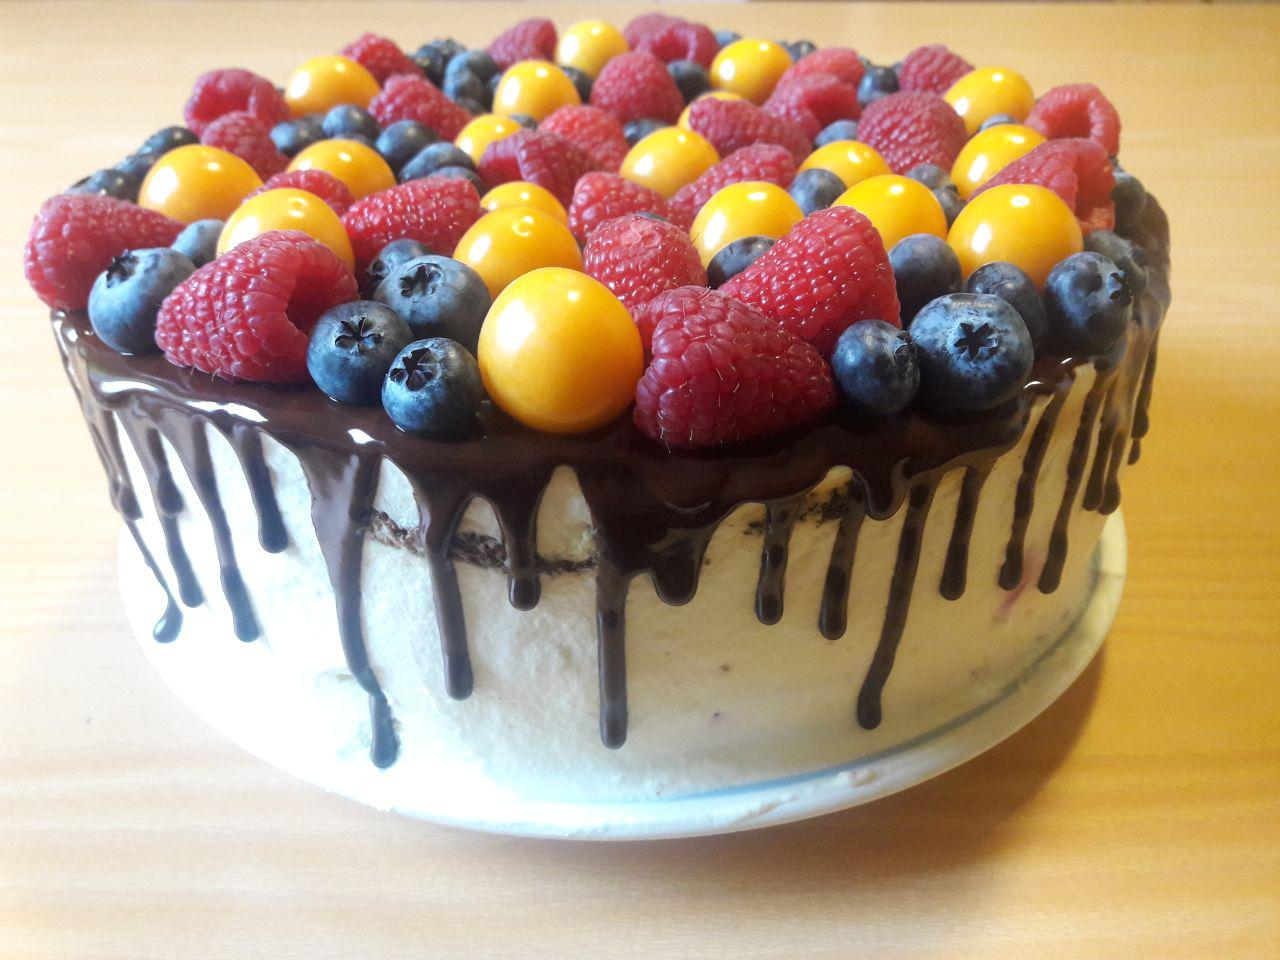
\includegraphics[width = 0.65\textwidth]{Bilder/torte1}
\caption{Leckere Torte}
\end{figure}

Um nur einen Bildausschnitt einzufügen, können die Parameter trim und clip zusammen verwendet werden. \verb+trim = left bottom right top+ gibt an, um wie viele cm jede Seite getrimmt werden soll.
Insgesamt ergibt sich dann für die Parameter bspw. \verb+[trim = 6cm 1cm 6cm 1cm, clip, width = 0.40\textwidth]+


\begin{figure}[h]
\centering
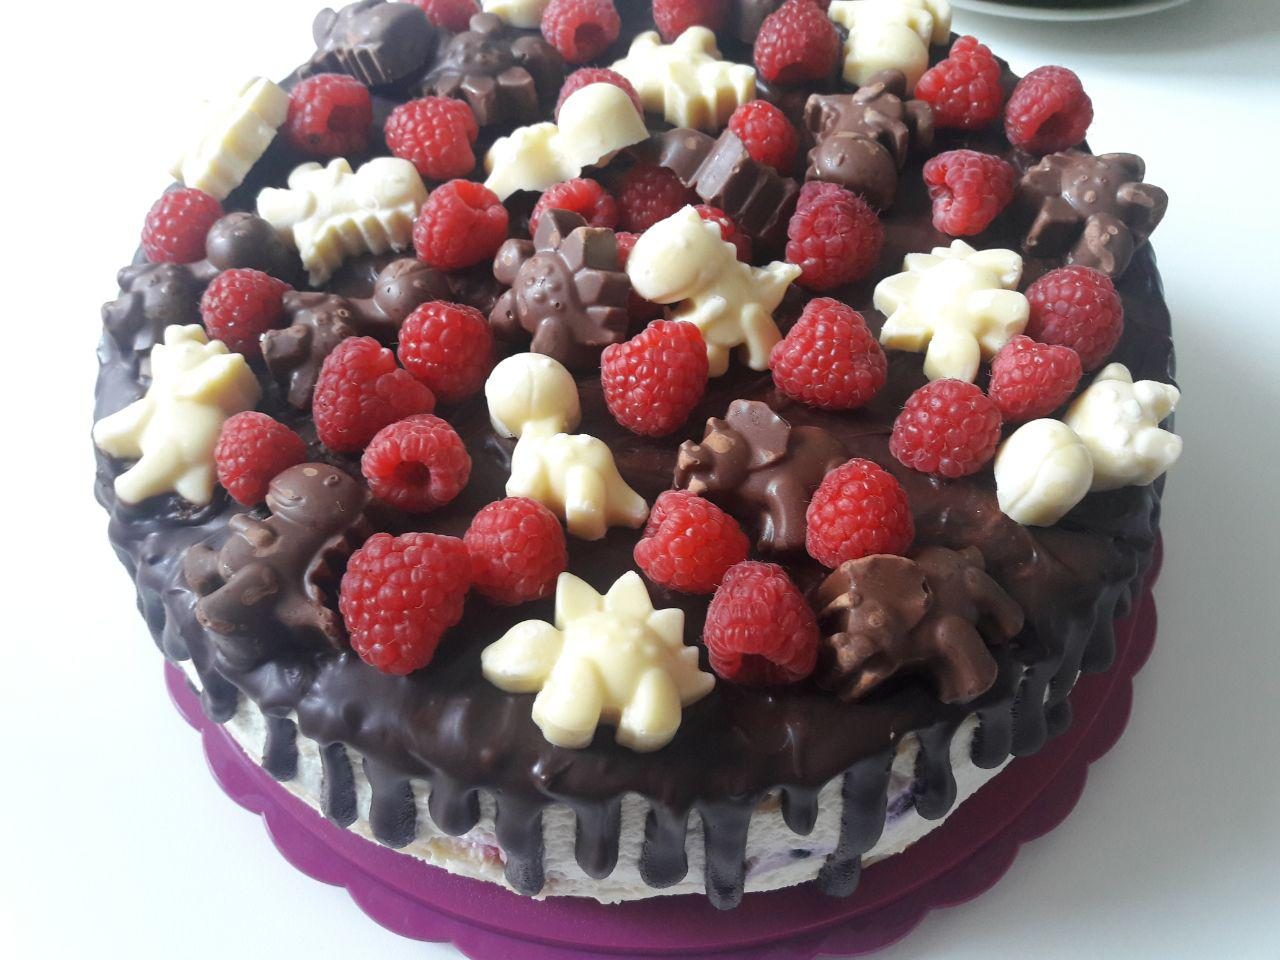
\includegraphics[trim = 6cm 3cm 6cm 1cm,clip , width = 0.35\textwidth]{Bilder/dinotorte}
\caption{Dino-Torte}
\end{figure}

Sollen (mehrere) ganze Seiten eines externen PDF-Dokuments eingefügt werden, kann der Befehl \verb+\includepdf[pages = {2,4,6-8}]{PDF_NAME}+ genutzt werden. 

\smallskip
Um zwei (oder mehr) Bilder nebeneinander auszugeben, können subfigures genutzt werden. Beispielcode dazu befindet sich in Anhang \ref{code_subfig}
\begin{figure}[h]
     \centering
     \begin{subfigure}[b]{0.55\textwidth}
         \centering
         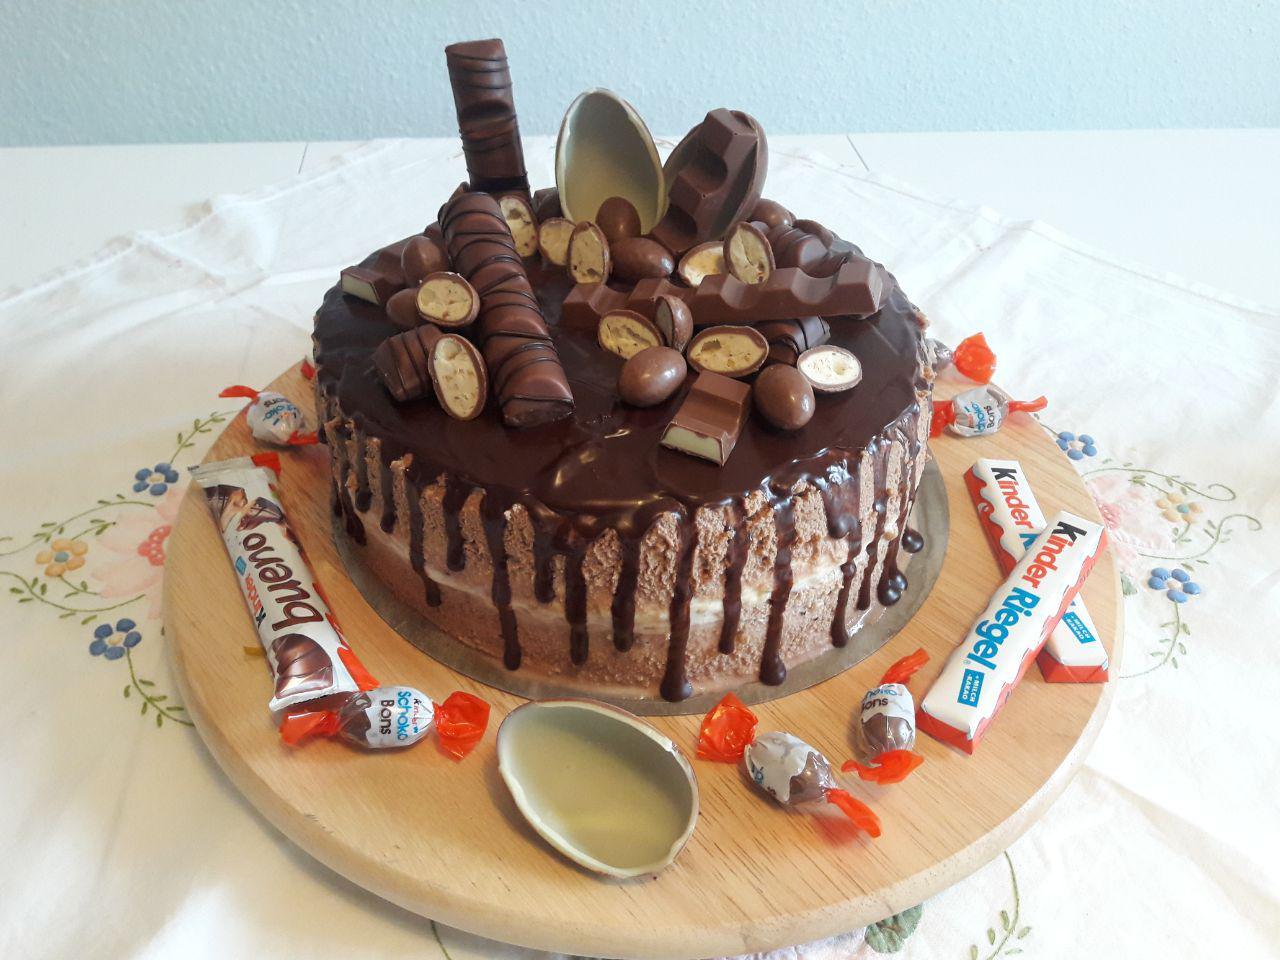
\includegraphics[width=\textwidth]{Bilder/kindertorte}
         \caption{Kinder-Torte}
         \label{fig:2_Bilder_Bild_1}
     \end{subfigure}
     \hfill
     \begin{subfigure}[b]{0.31\textwidth}
         \centering
         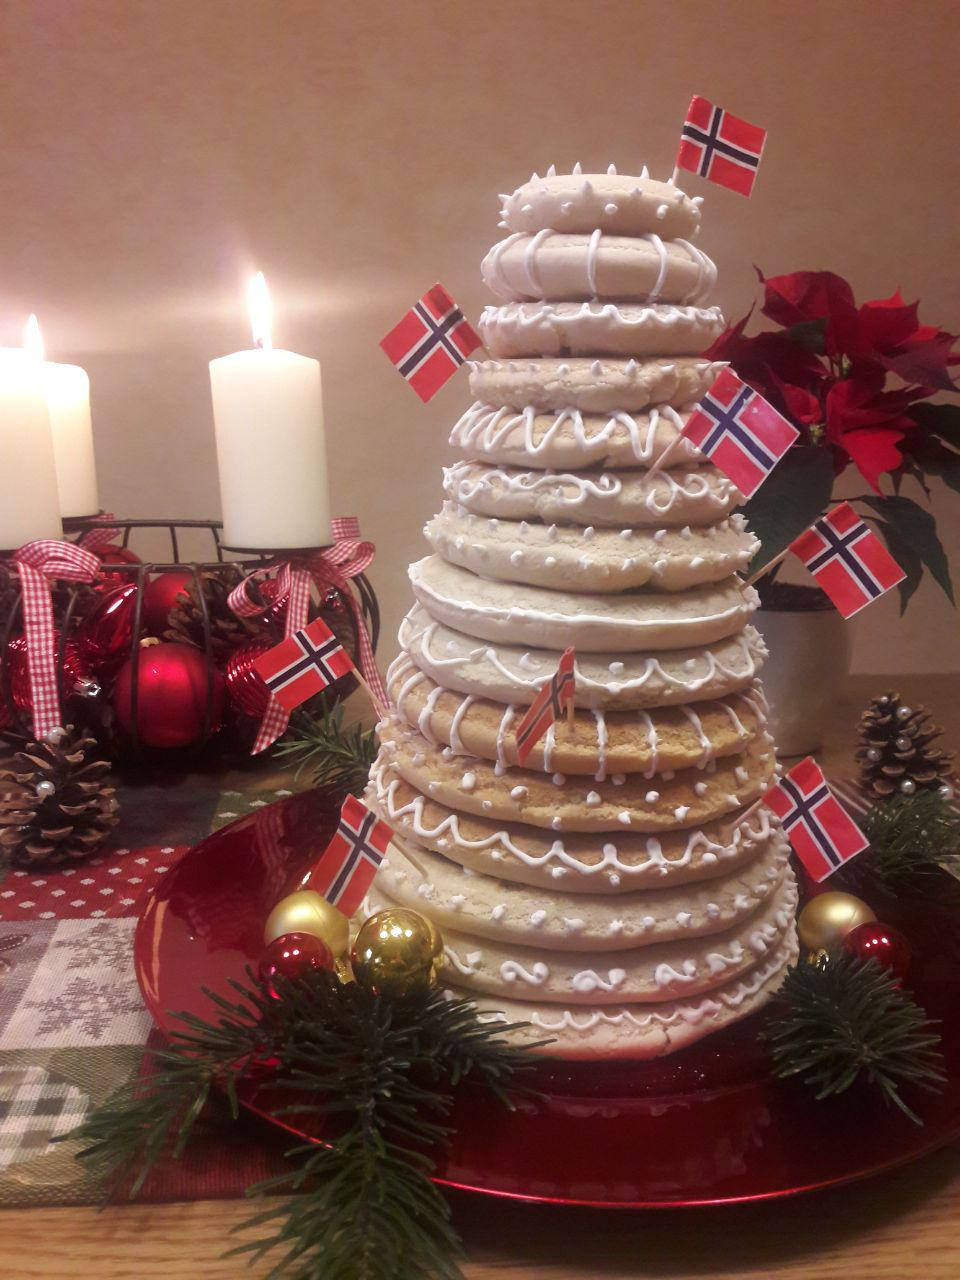
\includegraphics[width=\textwidth]{Bilder/kransekake}
         \caption{Kransekake}
         \label{fig:2_Bilder_Bild_2}
     \end{subfigure}
     \caption{Was schmeckt besser?}
\end{figure}

Für textumflossene Bilder kann die \texttt{floatingfigure}-Umgebung anstelle der \texttt{figure}-Umgebung genutzt werden. 
\verb+\begin{floatingfigure}[r\l\p]{width}+.


Dabei lässt sich die Platzierung des Bilds über die Parameter einstellen, r für rechts, l für links und p für Platzierung abhängig von der Seitenzahl.
\begin{floatingfigure}[l]{0.4\textwidth}
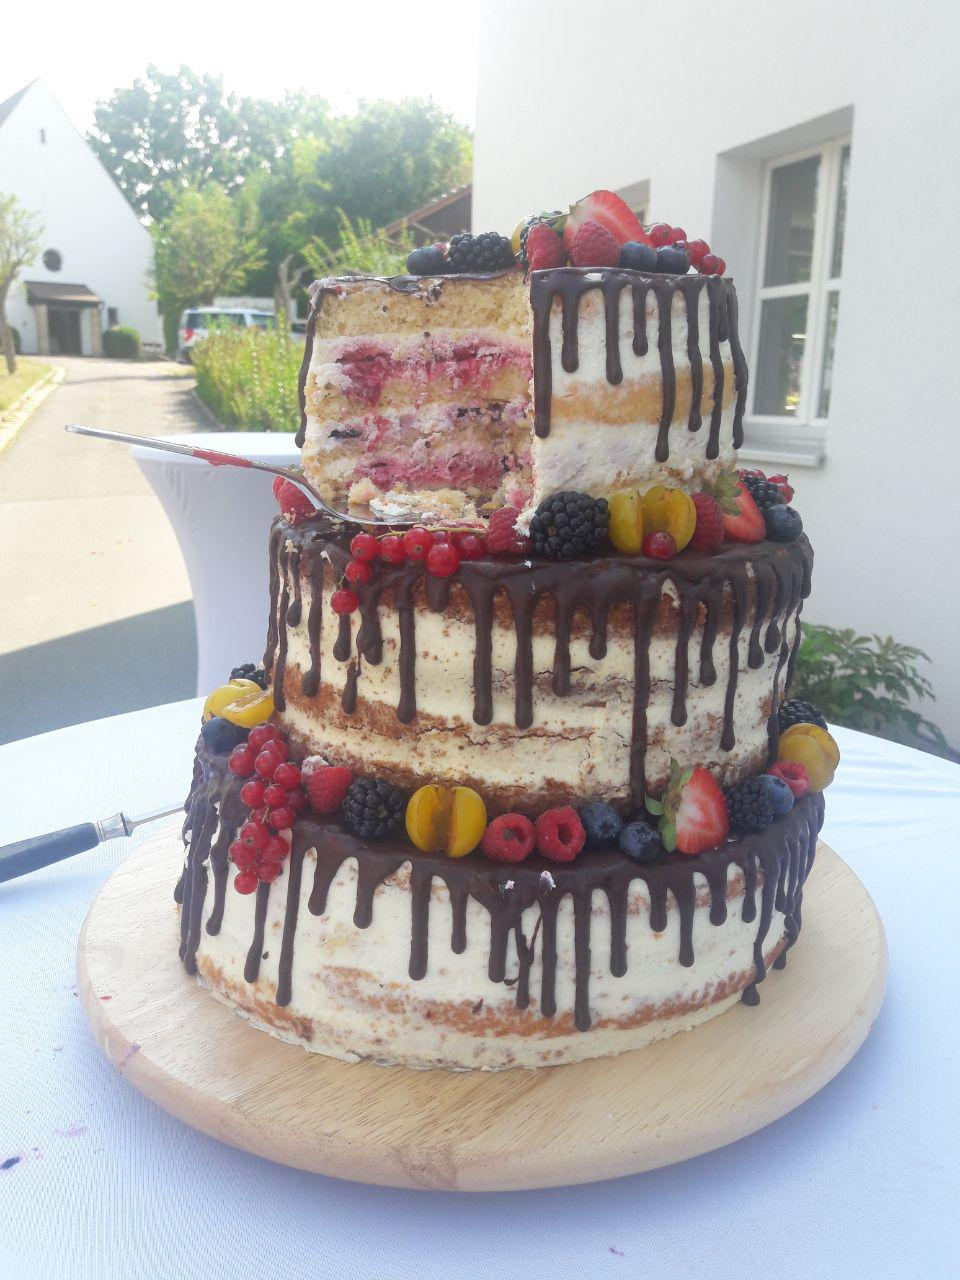
\includegraphics[width = 0.35\textwidth]{Bilder/hochzeitstorte}
\caption{Hochzeitstorte}
\end{floatingfigure} 
Mit width wird die Breite des Platzes, welcher für das Bild vorgesehen ist, festgelegt. 
Im Inneren der Umgebung wird das Bild wie gewohnt eingefügt. Auch eine Caption kann hier verwendet werden.
Die dort eingestellte Breite sollte zu der der floatingfigure passen. 
Schreibt man jetzt weiterhin Text, wird dieser neben dem Bild ausgegeben. Dabei sollte eine floatingfigure nicht zu nah an bspw. einer neuen Section platziert werden. Hier kommt es zur Kollision. Daher steht hier jetzt noch etwas unnötiger Text um den Abstand zum nächsten Kapitel zu vergrößern. Unnötiger Text und Kuchenbilder haben in Abschlussarbeiten aber in den meisten Fällen nichts zu suchen. Jetzt braucht es noch einen Satz, um das Bild vollständig zu überbrücken und zu zeigen, dass es danach wieder mit dem normalen Einzug weiter geht. 

Zur Einbindung von Formeln in Abbildungen empfiehlt sich Ti\textit{k}Z. Ein Editor zur Erstellung solcher Abbildung ist \emph{The Ipe extensible drawing editor} (\url{http://ipe.otfried.org/}). Durch Einbindung der \emph{ipe2tikz}-Erweiterung (\url{https://github.com/QBobWatson/ipe2tikz}) können so Vektorgrafiken erzeugt werden, die Formeln enthalten.
\begin{figure}[h]
	\centering
	\begin{tikzpicture}[scale=1.0, every node/.style={scale=1.0}]
	\tikzstyle{ipe stylesheet} = [
  ipe import,
  even odd rule,
  line join=round,
  line cap=butt,
  ipe pen normal/.style={line width=0.4},
  ipe pen heavier/.style={line width=0.8},
  ipe pen fat/.style={line width=1.2},
  ipe pen ultrafat/.style={line width=2},
  ipe pen normal,
  ipe mark normal/.style={ipe mark scale=3},
  ipe mark large/.style={ipe mark scale=5},
  ipe mark small/.style={ipe mark scale=2},
  ipe mark tiny/.style={ipe mark scale=1.1},
  ipe mark normal,
  /pgf/arrow keys/.cd,
  ipe arrow normal/.style={scale=7},
  ipe arrow large/.style={scale=10},
  ipe arrow small/.style={scale=5},
  ipe arrow tiny/.style={scale=3},
  ipe arrow normal,
  /tikz/.cd,
  ipe arrows, % update arrows
  <->/.tip = ipe normal,
  ipe dash normal/.style={dash pattern=},
  ipe dash dashed/.style={dash pattern=on 4bp off 4bp},
  ipe dash dotted/.style={dash pattern=on 1bp off 3bp},
  ipe dash dash dotted/.style={dash pattern=on 4bp off 2bp on 1bp off 2bp},
  ipe dash dash dot dotted/.style={dash pattern=on 4bp off 2bp on 1bp off 2bp on 1bp off 2bp},
  ipe dash normal,
  ipe node/.append style={font=\normalsize},
  ipe stretch normal/.style={ipe node stretch=1},
  ipe stretch normal,
  ipe opacity 10/.style={opacity=0.1},
  ipe opacity 30/.style={opacity=0.3},
  ipe opacity 50/.style={opacity=0.5},
  ipe opacity 75/.style={opacity=0.75},
  ipe opacity opaque/.style={opacity=1},
  ipe opacity opaque,
]
\begin{scope}[ipe stylesheet]
  \draw[shift={(232, 608)}, xscale=0.75]
    (0, 0) rectangle (64, -32);
  \draw
    (196, 592) circle[radius=4];
  \node[ipe node, anchor=north west]
     at (239, 596) {
       \begin{minipage}{60bp}\kern0pt
         Regler
       \end{minipage}
     };
  \draw[-{>[ipe arrow small]}]
    (164, 592)
     -- (192, 592);
  \draw[shift={(320.1, 608)}, xscale=0.7496]
    (0, 0) rectangle (64, -32);
  \node[ipe node, anchor=north west]
     at (328.1, 596) {
       \begin{minipage}{52bp}\kern0pt
         Strecke
       \end{minipage}
     };
  \node[ipe node]
     at (392, 599) {$y(t)$};
  \draw[shift={(400, 592)}, xscale=1.275, -{>[ipe arrow small]}]
    (0, 0)
     -- (0, -32)
     -- (-160, -32)
     -- (-160, -4);
  \filldraw[black]
    (400, 592) circle[radius=1];
  \draw[shift={(200.001, 592)}, xscale=2.6667, -{>[ipe arrow small]}]
    (0, 0)
     -- (12, 0);
  \draw[shift={(400.001, 592)}, xscale=2.6667, -{>[ipe arrow small]}]
    (0, 0)
     -- (12, 0);
  \draw[shift={(368.001, 592)}, xscale=2.6667]
    (0, 0)
     -- (12, 0);
  \draw[shift={(280.003, 592)}, xscale=3.3334, -{>[ipe arrow small]}]
    (0, 0)
     -- (12, 0);
  \node[ipe node]
     at (292, 599) {$u(t)$};
  \node[ipe node]
     at (208, 599) {$e(t)$};
  \node[ipe node]
     at (164, 599) {$w(t)$};
  \draw
    (200, 584)
     -- (204, 584);
  \draw[-{>[ipe arrow small]}]
    (344, 624)
     -- (344, 608);
  \node[ipe node]
     at (336, 631) {$z(t)$};
\end{scope}

	\end{tikzpicture}
	\caption{Standardregelkreis, erstellt mit dem Ti\textit{k}Z-Editor \emph{Ipe}} \label{fig:Standardregelkreis}
\end{figure}

\section{Tabellen}
Eine Anleitung zu Tabellen findet man hier: \url{https://www.overleaf.com/learn/latex/Tables}. 

Eine einfache Tabelle lässt sich mit Hilfe der \texttt{tabular}-Umgebung erzeugen: 

\begin{center}
\begin{verbatim}
\begin{table}[h]
\centering
\begin{tabular}{ c c c c }
\hline
 h1  & h2  & h3  & h4	\\ \hline
 t1  & t2  & t3  & t4	\\
 t5  & t6  & t7  & t8	\\  
 t9  & t10 & t11 & t12 \\ 
 t13 & t14 & t15 & t16 \\ \hline
\end{tabular}
\caption{einfache Tabelle}
\label{tab:tab1}
\end{table}
\end{verbatim}
\end{center}

\begin{table}[h]
\centering
\begin{tabular}{ c c c c }
\hline
 h1  & h2  & h3  & h4   \\ \hline
 t1  & t2  & t3  & t4   \\
 t5  & t6  & t7  & t8   \\  
 t9  & t10 & t11 & t12 	\\ 
 t13 & t14 & t15 & t16 	\\ \hline
\end{tabular}
\caption{einfache Tabelle}
\label{tab:tab1}
\end{table}

Die Parameter der tabular-Umgebung geben an, wie viele Spalten die Tabelle hat und wie diese jeweils ausgerichtet sind (l,c,r).  Durch Einfügen eines $\vert$ zwischen den Parametern lassen sich senkrechte Striche zwischen den Spalten einfügen. Für horizontale Trennstriche wird der Befehl \verb+\hline+ genutzt. Außerdem kann\verb+ \cline{x-y}+ genutzt werden, um den Strich nur von Spalte x bis y einzuzeichnen.


Um mehrere Reihen oder Spalten zusammenzufassen, können \verb+\multirow{•}{•}{•}+ und \verb+\multicolumn{•}{•}{•}+ verwendet werden. Dabei gibt der erste Parameter die Anzahl der Spalten/Reihen an die überspannt werden sollen, der zweite die Formatierung der Zelle, bzw. im Fall von Reihen die Breite der Spalte und der letzte den Inhalt der Zelle an. 

\begin{table}[h]
\centering
\begin{tabular}{ |c| c| c |}
\hline
\multicolumn{3}{|c|}{Kopf}\\
\hline
 & t2 & t3 \\ 
 \cline{2-3}
  \multirow{-2}*{t14} & t5 &\multicolumn{1}{c}{} \\  
 \cline{1-2}
 t7 &  t8 & \multicolumn{1}{c}{\multirow{-2}*{t69}}\\
\cline{1-2}
\end{tabular}
\caption{etwas ausgefallenere Tabelle}
\end{table}

Wie bei Bildern, lassen sich auch Tabellen durch \texttt{subtable} in der \texttt{table}-Umgebung nebeneinander darstellen. 
\newpage
\section{Formeln und Gleichungen}
Ein kleiner Einstieg ist hier: \url{https://www.overleaf.com/learn/latex/Mathematical_expressions} zu finden.
Für Gleichungen und Formeln gibt es eine Vielzahl verschiedener Möglichkeiten zur Umsetzung.

Einfache mathematische Ausdrücke, die in den Fließtext eingebunden werden sollen, können wie \(a=b\) in der Form \verb+\(a=b\)+ oder in einfachen Dollarzeichen \verb+$a=b$+ eingefügt werden.

Um die Formel in einer eigenen Zeile auszugeben, werden entweder doppelte Dollarzeichen \verb+$$a=b$$+ oder \verb+\[a=b\]+ verwendet.$$a=b$$ Alternativ kann auch die \texttt{equation}-Umgebung genutzt werden. 
\begin{equation}
a=b
\end{equation}
Wie bei der \texttt{figure}-Umgebung lässt sich auch hier ein Label vergeben. Unabhängig davon wird die Gleichungsnummer neben der Gleichung ausgegeben. Soll die \texttt{equation}-Umgebung ohne Nummerierung verwendet werden, kann diese mit \verb+\nonumber+ am Ende der Gleichung unterdrückt werden.  

\smallskip
Sollen mehrere Gleichungen untereinander ausgerichtet werden, kann die \texttt{align}-Umgebung genutzt werden. Dabei können mit \verb+&+ die Stellen markiert werden, an denen ausgerichtet werden soll. 
\begin{align}
a&=b-c\\
b-d&=d\cdot e\\
&=f
\end{align}

\begin{verbatim}
\begin{align}
a&=b-c\\
b-d&=d\cdot e\\
&=f
\end{align}
\end{verbatim}

Um nur eine Gleichungsnummer für alle Gleichungen zusammen auszugeben, wird der Befehl \verb+split+ verwendet.

\begin{align}
\begin{split}
a&=b-c\\
b-d&=d\cdot e\\
&=f
\end{split}
\end{align}

\begin{verbatim}
\begin{align}
\begin{split}
a&=b-c\\
b-d&=d\cdot e\\
&=f
\end{split}
\end{align}
\end{verbatim}


Für Matrizen werden je nach gewünschter Klammer \verb+pmatrix+ oder \verb+bmatrix+ verwendet. Als pmatrix besitzt die Matrix runde Klammern, als bmatrix eckige. 
\begin{align}\text{pmatrix:} &&
\begin{pmatrix}
a_{1,1} & \dots & a_{1,n}\\
\vdots & \ddots & \vdots \\
a_{m,1} & \dots & a_{m,n}
\end{pmatrix} \nonumber
\end{align}


\begin{align}\text{bmatrix:} &&
\begin{bmatrix}
a_{1,1} & \dots & a_{1,n}\\
\vdots & \ddots & \vdots \\
a_{m,1} & \dots & a_{m,n}
\end{bmatrix} \nonumber
\end{align}


Im Inneren sind die Matrizen wie Tabellen aufgebaut. Die Punkte lassen sich mit \verb+\dots+, \verb+\vdots+ und \verb+\ddots+ erzeugen.  


\chapter{Programmcode}
Programmcode lässt sich in der \verb+lstlisting+ Umgebung direkt schreiben oder über \verb+\lstinputlisting{PFAD/m_file.m}+ aus einer Datei einfügen. 

\begin{lstlisting}
i = 1; 
if ( i == 1){
	i--;
}
\end{lstlisting}


Verwendet man die definierten Styles \texttt{numbers} und \texttt{nonumbers}, lassen sich auch Zeilennummerierungen hinzufügen. Dazu setzt man \verb+\lstset{style = numbers}+.
\lstset{style = numbers}
\begin{lstlisting}
i = 1; 
if (i == 1){
	i--;
}
\end{lstlisting}

Code-Schnipsel, wie \lstinline!if(i == 1)! lassen sich auch direkt im Fließtext einbauen. Dazu wird \verb+\lstinline!CODE!+ verwendet.
Für Matlab-Code kann hier auch \verb+\mcode{CODE}+ genutzt werden. 

Außerdem kann mit \verb+\lstinputlisting{PFAD/DATEI}+ Code auch direkt aus Matlab-Dateien importiert werden. 

%%%%%%%%%%%%%%%%%%%%%%%%%%%%%%%%%%%%%%%%%%%%%%%%%%%%%%%%%%%%%%%%%%%%%%%%%
\cleardoublepage                                                        %
\listoffigures{\thispagestyle{pagenumberstyle}}                         %
\listoftables{\thispagestyle{pagenumberstyle}}                          %
\printbibliography{\thispagestyle{pagenumberstyle}}                     %
%\addchap{Anhang}                                                       %
\appendix                                                               %
%%%%%%%%%%%%%%%%%%%%%%%%%%%%%%%%%%%%%%%%%%%%%%%%%%%%%%%%%%%%%%%%%%%%%%%%%
\chapter{Anhang}

\section{Source Code der angepassten \textit{scatter}-Funktion}

%%
%% Julia definition (c) 2014 Jubobs
%%
\lstdefinelanguage{Julia}%
  {morekeywords={abstract,break,case,catch,const,continue,do,else,elseif,%
      end,export,false,for,function,immutable,import,importall,if,in,%
      macro,module,otherwise,quote,return,switch,true,try,type,typealias,%
      using,while},%
   sensitive=true,%
   alsoother={\$},%
   morecomment=[l]#,%
   morecomment=[n]{#=}{=#},%
   morestring=[s]{"}{"},%
   morestring=[m]{'}{'},%
}[keywords,comments,strings]%

\lstset{%
    language         = Julia,
    basicstyle       = \ttfamily,
    keywordstyle     = \bfseries\color{blue},
    stringstyle      = \color{magenta},
    commentstyle     = \color{ForestGreen},
    showstringspaces = false,
}

\label{code_subfig}
\lstset{language=Julia,style=nonumbers}
\begin{lstlisting}[language=Julia]
using CUDA
using ForwardDiff
using NNlibCUDA
using NNlib

_view(X, colons, k) = view(X, colons..., k...)
_view(X, colons, k::Union{Integer, CartesianIndex}) = 
    view(X, colons..., k)
 
maximum_dims(dims::AbstractArray{<:Integer}) = 
    (CUDA.findmax(dims)[1], )
maximum_dims(dims::AbstractArray{NTuple{N, T}}) where {N,T} = 
    ntuple(i -> CUDA.findmax(x->x[i], dims)[1], N)
maximum_dims(dims::AbstractArray{CartesianIndex{N}}) where {N} = 
    ntuple(i -> CUDA.findmax(x->x[i], dims)[1], N)
 
scatter_empty(op, T) = Base.reduce_empty(op, T)
scatter_empty(op::typeof(-), T) = zero(T)
scatter_empty(op::typeof(/), T) = one(T)
scatter_empty(op::typeof(min), T) = typemax(T)
scatter_empty(op::typeof(max), T) = typemin(T)


function NNlib.scatter(op::OP, src::AnyCuArray{Tsrc , Nsrc}, 
                       idx::AnyCuArray{Tidx, Nidx}; 
                       init = nothing, dstsize = nothing) 
                       where {Tsrc <: ForwardDiff.Dual{T, V, N},
                       Tidx,Nsrc,Nidx,OP} where {T, V, N}
    dims = Nsrc - Nidx 
    dstsz = isnothing(dstsize) ? 
            (size(src)[1:dims]..., 
            maximum_dims(idx)...) : dstsize 
    dst = similar(src, Tsrc, dstsz) 
    xinit = isnothing(init) ? scatter_empty(op, Tsrc) : init  
    fill!(dst, xinit) 
    
    return my_scatter(op, dst, src, idx)        
end

function my_scatter(op::OP, dst::AnyCuArray{Tdst, Ndst}, 
                            src::AnyCuArray{Tsrc, Nsrc} , 
                            idx::AnyCuArray{Tidx, Nidx}) 
                            where {Tsrc <: 
                            ForwardDiff.Dual{T, V, N}
                            ,Nsrc,Tidx,Nidx, Tdst, Ndst, OP} 
                            where {T, V, N}   


    dst_i = CuArray{V}(undef, (size(dst)..., N+1)) 
    src_i = CuArray{V}(undef, (size(src)..., N+1))
    
    # Create a tuple similar to Tidx but with one more element 
    if Tidx <: Tuple
        t = typeof(ntuple(x -> one(Tidx.parameters[1]), 
                              length(t.parameters)+1))
    else
        t = typeof(ntuple(x -> one(Tidx), 2))
    end

    # Allocate Space for the larger idx array
    # that is need for scatter!
    idx_i = CuArray{t}(undef, (size(idx)..., N+1))
    copy_dual_to_matrix(dst_i, dst)
    copy_dual_to_matrix(src_i, src)
    modify_index(idx_i, idx)

    NNlib.scatter!(op, dst_i, src_i, idx_i) 
    
    # Create an array that contains tuples 
    # for the partials of a Dual Number
    function f(x...)
        return x
    end
    tuples = f.([view(dst_i, 
             repeat([:], ndims(dst_i)-1)..., i) 
             for i in 2:(N+1)]...)


    # Copy the Result of the Computation 
    # into the destination array
    modify_dual(dst , view(dst_i, repeat([:], 
                ndims(dst_i)-1)..., 1), tuples)
    return dst
end

function copy_dual_to_matrix(dst_i, dst)
    kernel = CUDA.@cuda launch=false 
        copy_dual_to_matrix_kernel(dst_i, dst)
    config = CUDA.launch_configuration(kernel.fun; 
                                max_threads=256)
    threads = min(config.threads, length(dst_i))
    blocks = cld(length(dst_i), threads)
    
    kernel(dst_i, dst; threads=threads, blocks=blocks)
end

function copy_dual_to_matrix_kernel(src::CuDeviceArray{V}, 
            dst::CuDeviceArray{<: ForwardDiff.Dual{T, V, N}}) 
            where {T, V, N}
    index = threadIdx().x + (blockIdx().x - 1) * blockDim().x
   
    if index <= length(src) 
        # Convert the Linear Index index into Koordinates in src
        ci = CartesianIndices(src)
        loc = Tuple(ci[index])
        
        # Copy all values of a dual number 
        # into there respectiv location
        if loc[end] == 1
            src[loc...] = dst[loc[1:end-1]...].value 
        else 
            src[loc...] = 
                dst[loc[1:end-1]...].partials[loc[end]-1]
        end
    end
    return nothing
end

function modify_index(src, dst)
    kernel = CUDA.@cuda launch=false 
                modify_index_kernel(src, dst) 
    config = CUDA.launch_configuration(kernel.fun; 
                                max_threads=256)
    threads = min(length(src), config.threads)
    blocks = cld(length(src), threads)
    
    kernel(src, dst; threads=threads, blocks=blocks)
end

function modify_index_kernel(src::CuDeviceArray, 
                             dst::CuDeviceArray)
    index = threadIdx().x + (blockIdx().x - 1) * blockDim().x
    
    if index <= length(src)
        ci = CartesianIndices(src)
        loc = Tuple(ci[index])
        src[loc...] =  (dst[loc[1:end-1]...]..., loc[end])
    end
    return nothing
end

function modify_dual(dst, v, src)
    kernel = CUDA.@cuda launch=false dual_kernel(dst, v, src)
    config = CUDA.launch_configuration(kernel.fun; 
                                    max_threads=256)
    threads = min(length(dst), config.threads)
    blocks = cld(length(dst), threads)
    
    kernel(dst, v, src; threads=threads, blocks=blocks)
end

function dual_kernel(dst::CuDeviceArray{<: 
                ForwardDiff.Dual{T, V, N}}, 
                v::CuDeviceArray{V}, 
                src::CuDeviceArray{NTuple{N, V}}) 
                where {T, V, N}
    index = threadIdx().x + (blockIdx().x - 1) * blockDim().x
   
    if index <= length(src)
        ci = CartesianIndices(dst)
        loc = Tuple(ci[index])
        dst[loc...]= ForwardDiff.Dual{T, V, N}(v[loc...], 
                     ForwardDiff.Partials{N, V}(src[loc...]))
    end
    return nothing
end
\end{lstlisting}

\newpage

\section{Tabllen der Funktionierenden Impliziten Lösungs Algorithmen}
\label{solver_tabels}

\begin{table}[H]
    \centering
    
    \begin{tabular}{p{5cm}|c|p{5cm}}
        Name             & Funktionale & Fehler \\
        \hline\hline        
        ImplicitEuler    & true        & \\ 
        ImplicitMidpoint & true        & \\ 
        Trapezoid        & true        & \\ 
        TRBDF2           & true        & \\ 
        SDIRK2           & true        & \\ 
        Kvaerno3         & true        & \\ 
        KenCarp3         & true        & \\ 
        Cash4            & true        & \\ 
        Hairer4          & true        & \\ 
        Hairer42         & true        & \\ 
        Kvaerno4         & true        & \\ 
        KenCarp4         & true        & \\ 
        KenCarp47        & true        & \\ 
        Kvaerno5         & true        & \\ 
        KenCarp5         & true        & \\ 
        KenCarp58        & true        & \\       
    \end{tabular}
    \caption{SDIRK Methods}
    \label{tab:my_label}
\end{table}

\begin{table}[H]
    \centering

    \begin{tabular}{p{5cm}|c|p{5cm}}
        Name & Funktionale & Fehler \\
        \hline\hline
        RadauIIA3 & false & Error: DimensionMismatch: arguments must have the same number of rows \\
        RadauIIA5 & false & Error: DimensionMismatch: arguments must have the same number of rows \\
    \end{tabular}
    \caption{Fully-Implicit Runge-Kutta Methods}
    \label{tab:my_label}
\end{table}

\begin{table}[H]
    \centering

    \begin{tabular}{p{5cm}|c|p{5cm}}
        Name & Funktionale & Fehler \\
        \hline\hline
        PDIRK44 & false & Error: `@threads :static` cannot be used concurrently or nested \\
    \end{tabular}
    \caption{Parallel Diagonally Implicit Runge-Kutta Methods}
    \label{tab:my_label}
\end{table}

\begin{table}[H]
    \centering

    \begin{tabular}{p{5cm}|c|p{5cm}}
        Name & Funktionale & Fehler \\
        \hline\hline
        ROS3P     & true & \\ 
        Rodas3    & true & \\ 
        RosShamp4 & true & \\ 
        Veldd4    & true & \\ 
        Velds4    & true & \\ 
        GRK4T     & true & \\ 
        GRK4A     & true & \\ 
        Ros4LStab & true & \\ 
        Rodas4    & true & \\ 
        Rodas42   & true & \\ 
        Rodas4P   & true & \\ 
        Rodas4P2  & true & \\ 
        Rodas5    & true & \\ 
    \end{tabular}
    \caption{Rosenbrock Methods}
    \label{tab:my_label}
\end{table}

\begin{table}[H]
    \centering

    \begin{tabular}{p{5cm}|c|p{5cm}}
        Name & Funktional & Fehler \\
        \hline\hline
        Rosenbrock23     & true & \\                                                                                                                          ║
        Rosenbrock32     & true & \\                                                                                                                          ║
        RosenbrockW6S4OS & true & \\                                                                                                                      ║
        ROS34PW1a        & true & \\                                                                                                                             ║
        ROS34PW1b        & true & \\                                                                                                                             ║
        ROS34PW2    & true & \\                                                                                                                              ║
        ROS34PW3         & true & \\            
    \end{tabular}
    \caption{Rosenbrock-W Methods}
    \label{tab:my_label}
\end{table}

\begin{table}[H]
    \centering

    \begin{tabular}{p{10cm}|c|p{1cm}}
        Name & Funktionale & Fehler \\
        \hline\hline
            ImplicitEulerExtrapolation & true & \\ 
            ImplicitDeuflhardExtrapolation & true & \\ 
            ImplicitHairerWannerExtrapolation & true & \\ 
    \end{tabular}
    \caption{Parallelized Implicit Extrapolation Methods}
    \label{tab:my_label}
\end{table}

\begin{table}[H]
    \centering

    \begin{tabular}{p{5cm}|c|p{5cm}}
        Name & Funktionale & Fehler \\
        \hline\hline
        PDIRK44 & false & Error: `@threads :static` cannot be used concurrently or nested \\     
    \end{tabular}
    \caption{Parallelized DIRK Methods}
    \label{tab:my_label}
\end{table}

\begin{table}[H]
    \centering

    \begin{tabular}{p{5cm}|c|p{5cm}}
        Name & Funktionale & Fehler \\
        \hline\hline
        LawsonEuler  & false & Error: ArgumeError: Caching can only be used with SplitFunction \\
        NorsettEuler & false & Error: ArgumeError: Caching can only be used with SplitFunction \\
        ETD2         & false & Error: type ODEFunction has no field f1 \\
        ETDRK2       & false & Error: ArgumeError: Caching can only be used with SplitFunction \\
        ETDRK3       & false & Error: ArgumeError: Caching can only be used with SplitFunction \\
        ETDRK4       & false & Error: ArgumeError: Caching can only be used with SplitFunction \\
        HochOst4     & false & Error: ArgumeError: Caching can only be used with SplitFunction \\
    \end{tabular}
    \caption{Exponential Runge-Kutta Methods}
    \label{tab:my_label}
\end{table}

\begin{table}[H]
    \centering

    \begin{tabular}{p{5cm}|c|p{5cm}}
        Name & Funktionale & Fehler \\
        \hline\hline
        Exp4      & false & Error: AssertiError: Dimension mismatch \\
        EPIRK4s3A & false & Error: AssertiError: Dimension mismatch \\
        EPIRK4s3B & false & Error: AssertiError: Dimension mismatch \\
        EPIRK5P1  & false & Error: AssertiError: Dimension mismatch \\
        EPIRK5P2  & false & Error: AssertiError: Dimension mismatch \\
        EPIRK5s3  & false & Error: DimensionMismatch: tried to assign 2×1896 array to 3792×1 destination \\
        EXPRB53s3 & false & Error: AssertiError: Dimension mismatch \\
    \end{tabular}
    \caption{Exponential Propagation Iterative Runge-Kutta Methods}
    \label{tab:my_label}
\end{table}

\begin{table}[H]
    \centering

    \begin{tabular}{p{5cm}|c|p{5cm}}
        Name & Funktionale & Fehler \\
        \hline\hline
        Exprb32 & false & Error: DimensionMismatch: array could not be broadcast to match destination \\
        Exprb43 & false & Error: DimensionMismatch: A has dimensions (3792,3792) but B has dimensions (2,1896) \\       
    \end{tabular}
    \caption{Adative Exponential Rosenbrock Methods}
    \label{tab:my_label}
\end{table}

\begin{table}[H]
    \centering

    \begin{tabular}{p{5cm}|c|p{5cm}}
        Name & Funktionale & Fehler \\
        \hline\hline
        QNDF1 & true   & \\
        QBDF1 & true   & \\
        ABDF2 & true   & \\
        QNDF2 & true   & \\
        QBDF2 & true   & \\
        QNDF  & false  & Erros DimensionMissmatch \\
        QBDF  & false  & Erros DimensionMismatch \\
        MEBDF2& false  & Works but slow \\
        FBDF  & false  & Doesn work on gpu because scalar indexing \\
    \end{tabular}
    \caption{Mutlistep Methods}
    \label{tab:my_label}
\end{table}

\begin{table}[H]
    \centering

    \begin{tabular}{p{5cm}|c|p{5cm}}
        Name & Funktionale & Fehler \\
        \hline\hline
        SSPSDIRK2 & false & Error: MethError: Cannot `convert` an object of type Float32 to an object of type CUDA.CuArray{Float32, 2, CUDA.Mem.DeviceBuffer}║ \\        
    \end{tabular}
    \caption{Implicit Strong-Stability Preserving Runge-Kutta Methods for Hyperbolic PDEs}
    \label{tab:my_label}
\end{table}
                                                   
\chapter*{Erklärung}
Die vorliegende Arbeit habe ich selbstständig ohne Benutzung anderer als der
angegebenen Quellen angefertigt. Alle Stellen, die wörtlich oder sinngemäß
aus veröffentlichten Quellen entnommen wurden, sind als solche
kenntlich gemacht. Die Arbeit ist in gleicher oder ähnlicher Form oder
auszugsweise im Rahmen einer oder anderer Prüfungen noch nicht vorgelegt
worden.
\\[2cm]
Augsburg, den \eingereicht\hfill \namedesautors                                      
%%%%%%%%%%%%%%%%%%%%%%%%%%%%%%%%%%%%%%%%%%%%%%%%%%%%%%%%%%%%%%%%%%%%%%%%%
\end{document}                                                          %
%%%%%%%%%%%%%%%%%%%%%%%%%%%%%%%%%%%%%%%%%%%%%%%%%%%%%%%%%%%%%%%%%%%%%%%%%